\documentclass[letterpaper, 12pt]{report}
%%%%%%%%%%%%%%%%%%%%%%%%%%%%%%%%%%%%%%%%%%%%%%%%%%%%%%%%%%%%%%%%%%%%%%%%%%%%%%%%%%%%%%%%%%%%%%%%%%%%%
\usepackage{amsmath}
\usepackage{amssymb}
\usepackage{fullpage}
\usepackage[usenames,dvipsnames]{color}
\usepackage{setspace}
\usepackage{url}
\usepackage{hyperref}
\usepackage{graphicx}
%%%%%%%%%%%%%%%%%%%%%%%%%%%%%%%%%%%%%%%%%%%%%%%%%%%%%%%%%%%%%%%%%%%%%%%%%%%%%%%%%%%%%%%%%
\newcommand{\red}[1]{{\color{red} #1}}
\newcommand{\blue}[1]{{\color{blue} #1}}
\newcommand{\green}[1]{{\color{ForestGreen} #1}}
\newcommand{\magenta}[1]{{\color{magenta} #1}}
\newcommand{\cyan}[1]{{\color{cyan} #1}}
\newcommand{\yellow}[1]{{\color{Dandelion} #1}}
\newcommand{\black}[1]{{\color{black} #1}}
\newcommand{\gray}[1]{{\color{Gray} #1}}
\renewcommand{\thechapter}{\Alph{chapter}}
%%%%%%%%%%%%%%%%%%%%%%%%%%%%%%%%%%%%%%%%%%%%%%%%%%%%%%%%%%%%%%%%%%%%%%%%%%%%%%%%%%%%%%%%%
\begin{document}
%%%%%%%%%%%%%%%%%%%%%%%%%%%%%%%%%%%%%%%%%%%%%%%%%%%%%%%%%%%%%%%%%%%%%%%%%%%%%%%%%%%%%%%%%
\title{\textsc{PHYS 207L Data Analysis Guides}}
\author{M.E. Irizarry-Gelp\'{i}}
\date{\today}
%%%%%%%%%%%%%%%%%%%%%%%%%%%%%%%%%%%%%%%%%%%%%%%%%%%%%%%%%%%%%%%%%%%%%%%%%%%%%%%%%%%%%%%%%
\maketitle
\tableofcontents
%%%%%%%%%%%%%%%%%%%%%%%%%%%%%%%%%%%%%%%%%%%%%%%%%%%%%%%%%%%%%%%%%%%%%%%%%%%%%%%%%%%%%%%%%
% Copyright 2018 Melvin Eloy Irizarry-Gelpí
\chapter{Working with Spreadsheets}
%%%%%%%%%%%%%%%%%%%%%%%%%%%%%%%%%%%%%%%%%%%%%%%%%%%%%%%%%%%%%%%%%%%%%%%%%%%%%%%%
In this experiment you will gain experience using spreadsheets to analyze and visualize data.
%%%%%%%%%%%%%%%%%%%%%%%%%%%%%%%%%%%%%%%%%%%%%%%%%%%%%%%%%%%%%%%%%%%%%%%%%%%%%%%%
\section{Preliminary}
%%%%%%%%%%%%%%%%%%%%%%%%%%%%%%%%%%%%%%%%%%%%%%%%%%%%%%%%%%%%%%%%%%%%%%%%%%%%%%%%
Spreadsheet technology is commonly available in the form of software like Microsoft Excel, LibreOffice Calc, or Google Sheets.

Excel is part of Microsoft Office, and you usually need a license to use it. Calc is part of LibreOffice, which is a free version of Office. Both Excel and Calc can be used as apps in your desktop or laptop. Google Sheets is very similar, but can be used through a web browser like Chrome or Firefox. All three share a common set of basic functionality, which is what we will need.

Since Google Sheets is available as part of the suit of apps provided by the College, and it works the same way in Windows, Mac OS X, and Linux, I will be using Google Sheets for all my analysis work. Use of Google Sheets is not mandatory but encouraged.

In this experiment you will get a first encounter with using spreadsheets to analyze physics data. You will
\begin{enumerate}
    \item Import data into a spreadsheet
    \item Make charts for visualization
    \item Use built-in functions to analyze the data
    \item Make a table with results
\end{enumerate}
%%%%%%%%%%%%%%%%%%%%%%%%%%%%%%%%%%%%%%%%%%%%%%%%%%%%%%%%%%%%%%%%%%%%%%%%%%%%%%%%
\section{Experiment}
%%%%%%%%%%%%%%%%%%%%%%%%%%%%%%%%%%%%%%%%%%%%%%%%%%%%%%%%%%%%%%%%%%%%%%%%%%%%%%%%
There is no actual experiment to collect the data. You will work with two data files, each describing a different hypothetical experiment. Although the data in each file was generated with a computer program, it is similar to some of the data that you will collect later in the semester from sensors during an experiment.
%%%%%%%%%%%%%%%%%%%%%%%%%%%%%%%%%%%%%%%%%%%%%%%%%%%%%%%%%%%%%%%%%%%%%%%%%%%%%%%%
\subsection{Mass Measurement}
%%%%%%%%%%%%%%%%%%%%%%%%%%%%%%%%%%%%%%%%%%%%%%%%%%%%%%%%%%%%%%%%%%%%%%%%%%%%%%%%
This experiment consists of a hypothetical \textbf{mass} measurement taken over \textbf{time}. Three mass values are measured. First, between the starting time $t = t_{I}$ and $t = t_{1}$ a \textbf{baseline mass} measurement $m_{B}$ is taken to calibrate the sensor. Then, between $t = t_{1}$ and $t = t_{2}$ the \textbf{mass 1} measurement $m_{1}$ is taken. Finally, between $t = t_{2}$ and $t = t_{F}$ the \textbf{mass 2} measurement $m_{2}$ is taken. That is:
\begin{itemize}
    \item $t_{I} < t < t_{1}$: Baseline mass measurement $m_{B}$
    \item $t_{1} < t < t_{2}$: Mass 1 measurement $m_{1}$
    \item $t_{2} < t < t_{F}$: Mass 2 measurement $m_{2}$
\end{itemize}
You need to provide the best estimate for the three mass values from the data.

Although this is a measurement over time, we will treat each time measurement as \textbf{independent}. That is, this hypothetical sensor is repeatedly measuring the same quantity, but due to noise, it cannot provide the same result each time. The main challenge is to deal with this noise. Which value to report? The first one? The last one? The one in the middle of the experiment? One value chosen at random?
%%%%%%%%%%%%%%%%%%%%%%%%%%%%%%%%%%%%%%%%%%%%%%%%%%%%%%%%%%%%%%%%%%%%%%%%%%%%%%%%
\subsection{Velocity Measurement}
%%%%%%%%%%%%%%%%%%%%%%%%%%%%%%%%%%%%%%%%%%%%%%%%%%%%%%%%%%%%%%%%%%%%%%%%%%%%%%%%
This experiment consist of a hypothetical \textbf{velocity} measurement taken over \textbf{time}. You need to see if there exist a relationship between the velocity values and the time values. In order to answer this, it will be helpful to make a chart of velocity versus time.
%%%%%%%%%%%%%%%%%%%%%%%%%%%%%%%%%%%%%%%%%%%%%%%%%%%%%%%%%%%%%%%%%%%%%%%%%%%%%%%%
\section{Analysis}
%%%%%%%%%%%%%%%%%%%%%%%%%%%%%%%%%%%%%%%%%%%%%%%%%%%%%%%%%%%%%%%%%%%%%%%%%%%%%%%%
There are two parts. But before the analysis you need to setup your environment.
%%%%%%%%%%%%%%%%%%%%%%%%%%%%%%%%%%%%%%%%%%%%%%%%%%%%%%%%%%%%%%%%%%%%%%%%%%%%%%%%
\subsection{Setup for Mass Measurement}
%%%%%%%%%%%%%%%%%%%%%%%%%%%%%%%%%%%%%%%%%%%%%%%%%%%%%%%%%%%%%%%%%%%%%%%%%%%%%%%%
Here are some steps to follow before you can analyze the mass data.
%%%%%%%%%%%%%%%%%%%%%%%%%%%%%%%%%%%%%%%%%%%%%%%%%%%%%%%%%%%%%%%%%%%%%%%%%%%%%%%%
\subsubsection{Obtain the data}
%%%%%%%%%%%%%%%%%%%%%%%%%%%%%%%%%%%%%%%%%%%%%%%%%%%%%%%%%%%%%%%%%%%%%%%%%%%%%%%%
This step involves obtaining the data. For this activity, I will provide you with data. Later in the semester you will collect your own data from an experiment!

You can find the data file \texttt{mass.tsv} in Canvas. Download the file and add it to your working directory (either in your own computer or to your Google Drive in the cloud). It is a good idea to organize your files by lab number, so this data file could be inside a folder named \texttt{lab00-intro}.

The file extension \texttt{.tsv} means \textbf{Tab Separated Values}, meaning that each line consist of values separated by tab spaces. The files generated by the Vernier data collection devices that we are going to use will be in a similar format.
%%%%%%%%%%%%%%%%%%%%%%%%%%%%%%%%%%%%%%%%%%%%%%%%%%%%%%%%%%%%%%%%%%%%%%%%%%%%%%%%
\subsubsection{View the data}
%%%%%%%%%%%%%%%%%%%%%%%%%%%%%%%%%%%%%%%%%%%%%%%%%%%%%%%%%%%%%%%%%%%%%%%%%%%%%%%%
This step is a sanity check: you want to take a \textbf{quick glimpse} at the data that you just obtained to make sure that everything is going well.

You can use a simple \textbf{text editor} like Notepad (Windows) or TextEdit (OS X) to open and view the data. You should see about 600 lines of text, each with two numerical values. The first line is a \textbf{header} and contains information about the data below. In our case, the header says that the first column is a quantity representing \textbf{time} measured in \textbf{seconds} (s), and the second column is a quantity representing \textbf{mass} measured in \textbf{grams} (g). Both the \textbf{names} and the \textbf{units} of each quantity are equally important.

Note that Microsoft Word and/or Google Docs are not simple text editors but complicated \textbf{word processors}. A text editor only allows simple editing like adding, changing, or removing characters in a text. A word processor allows you to format a text into different pages, make text bold, change fonts, etcetera. If you use a word processor to view data, the data will get split into multiple pages, and also might acquire unnecessary formating.

As you can see, a single data file with hundreds of rows can correspond to dozens of pages of paper. For this reason, \textbf{you should not include raw data files in your lab reports}. It is more useful (and less wasteful) to include the raw data in a spreadsheet that is shared electronically.
%%%%%%%%%%%%%%%%%%%%%%%%%%%%%%%%%%%%%%%%%%%%%%%%%%%%%%%%%%%%%%%%%%%%%%%%%%%%%%%%
\subsubsection{Import the data}
%%%%%%%%%%%%%%%%%%%%%%%%%%%%%%%%%%%%%%%%%%%%%%%%%%%%%%%%%%%%%%%%%%%%%%%%%%%%%%%%
This step involves putting the data into Google Sheets or Excel for analysis.

If you \textbf{copy and paste} the data directly into a spreadsheet, you will probably end with a \textbf{single column} of data. But if you look closely, the data involves two columns of numbers. A single column with spaced values is not useful in a spreadsheet.

Instead of copying and pasting the data, it is better to \textbf{import} it. In Google Sheets, you can do this by going to
\begin{center}
    \texttt{File > Import}
\end{center}
Find your file. As import location, choose \texttt{Insert new sheet(s)}. You do not need to change any other import setting. After this you should see a spreadsheet with \textbf{two columns} of data. Column \texttt{A} should be time, and column \texttt{B} should be mass.

I will refer to this sheet with the raw data by the name \texttt{RawData}. You can change the name of a sheet by double-clicking on the tab near the bottom of the screen.
%%%%%%%%%%%%%%%%%%%%%%%%%%%%%%%%%%%%%%%%%%%%%%%%%%%%%%%%%%%%%%%%%%%%%%%%%%%%%%%%
\subsubsection{Visualize the full data}
%%%%%%%%%%%%%%%%%%%%%%%%%%%%%%%%%%%%%%%%%%%%%%%%%%%%%%%%%%%%%%%%%%%%%%%%%%%%%%%%
This step involves making a chart in order to obtain an initial visualization of the full data.

Before any analysis is done on the new data, it is always useful to make a quick visualization. You can do this by selecting the two columns with data (hold the Shift key), and clicking on \texttt{Insert Chart}. By default, Google Sheets will provide you with a \textbf{line chart}. This is not necessarily the best option for our kind of data, so change the \texttt{Chart Type} to a \textbf{scatter chart} with points instead of a line. I find it convenient to change the default settings for the size of the points, in order to obtain a better graph. You can double-click on a chart to access the \texttt{Chart editor} menu, and then going to
\begin{center}
    \texttt{Chart Editor > Customize > Series > Point Size}
\end{center}
and changing the value from \texttt{7px} to \texttt{2px}.

You should see three horizontal regions with points. Each region corresponds to a different measurement. Looking at the graph you can learn that
\begin{itemize}
    \item The baseline measurement happens between $t = 0$ s and $t = 10$ s
    \item The mass 1 measurement happens between $t = 10$ s and $t = 20$ s
    \item The mass 2 measurement happens between $t = 20$ s and $t = 30$ s
\end{itemize}
By just looking at the graph, you have already learned something useful about the data.
%%%%%%%%%%%%%%%%%%%%%%%%%%%%%%%%%%%%%%%%%%%%%%%%%%%%%%%%%%%%%%%%%%%%%%%%%%%%%%%%
\subsubsection{Separate the data}
%%%%%%%%%%%%%%%%%%%%%%%%%%%%%%%%%%%%%%%%%%%%%%%%%%%%%%%%%%%%%%%%%%%%%%%%%%%%%%%%
Since there are three different measurements, it would be useful to work on three \textbf{separate sheets}. Add three empty sheets and give them useful names like \texttt{Baseline}, \texttt{One}, and \texttt{Two} or something similar that will help you remember later what each sheet corresponds to.

The first row on each sheet should be a header with the name and unit of each quantity. You can copy and paste the header row in \texttt{RawData}. The sheet with the baseline measurement should have the data between times 0 s and 10 s. You can select this region in \texttt{RawData}, copy it, and paste it to the \texttt{Baseline} sheet. Note that the baseline measurement actually ends at the 9.95 s time value. After doing this, the \texttt{Baseline} sheet should have about 200 rows with data. Similar steps can be taken with the other two measurements.
%%%%%%%%%%%%%%%%%%%%%%%%%%%%%%%%%%%%%%%%%%%%%%%%%%%%%%%%%%%%%%%%%%%%%%%%%%%%%%%%
\subsubsection{Visualize each segment}
%%%%%%%%%%%%%%%%%%%%%%%%%%%%%%%%%%%%%%%%%%%%%%%%%%%%%%%%%%%%%%%%%%%%%%%%%%%%%%%%
After separating each segment, it will be helpful to make a scatter chart for each portion, in order to get a better idea of how each segment looks up close.

Each chart should have a \textbf{title}, and \textbf{labeled horizontal and vertical axes}. You can double-click on a chart to access the \texttt{Chart editor} menu. The title can be changed under
\begin{center}
    \texttt{Chart editor > Chart \& axis titles > Type}
\end{center}
and choose the \texttt{Chart title} option to add a title to the chart. A good title would be something along the lines of ``Baseline Measurement'' in order to provide context. You can add a label to the horizontal axis by choosing \texttt{Horizontal axis title} instead. A good axis label will include the \textbf{name of the quantity} and the \textbf{units} being used to measure it.

Other useful changes to the default settings are to reduce the size of the points, and to remove the legend, since only one quantity is being plotted.
%%%%%%%%%%%%%%%%%%%%%%%%%%%%%%%%%%%%%%%%%%%%%%%%%%%%%%%%%%%%%%%%%%%%%%%%%%%%%%%%
\subsection{Descriptive Statistics for Mass Measurement}
%%%%%%%%%%%%%%%%%%%%%%%%%%%%%%%%%%%%%%%%%%%%%%%%%%%%%%%%%%%%%%%%%%%%%%%%%%%%%%%%
The steps in this section apply to each of the three segments in the data, but \textbf{I will use the baseline segment} for illustration purposes.
%%%%%%%%%%%%%%%%%%%%%%%%%%%%%%%%%%%%%%%%%%%%%%%%%%%%%%%%%%%%%%%%%%%%%%%%%%%%%%%%
\subsubsection{Minimum}
%%%%%%%%%%%%%%%%%%%%%%%%%%%%%%%%%%%%%%%%%%%%%%%%%%%%%%%%%%%%%%%%%%%%%%%%%%%%%%%%
Since the mass values are spread over a region, it is useful to known what is the smallest mass measurement in the segment, or \textbf{minimum}. This can be found by using the \texttt{MIN} function via
\begin{center}
    \texttt{=MIN(MassB)}
\end{center}
Note the equal sign in the beginning. In my case, the minimum value in the baseline segment is 0.468206 g.
%%%%%%%%%%%%%%%%%%%%%%%%%%%%%%%%%%%%%%%%%%%%%%%%%%%%%%%%%%%%%%%%%%%%%%%%%%%%%%%%
\subsubsection{25th Percentile}
%%%%%%%%%%%%%%%%%%%%%%%%%%%%%%%%%%%%%%%%%%%%%%%%%%%%%%%%%%%%%%%%%%%%%%%%%%%%%%%%
The \textbf{25th percentile} is the mass value measured that is larger than one quarter of all of the mass values in the data. This can be computed using the \texttt{PERCENTILE} function via
\begin{center}
    \texttt{=PERCENTILE(MassB, 0.25)}
\end{center}
Equivalently, this can be computed using the \texttt{QUARTILE} function via
\begin{center}
    \texttt{=QUARTILE(MassB, 1)}
\end{center}
The ``1'' here indicates the \textbf{first quartile}, which is another name for the 25th percentile. In my case, the 25th percentile in the baseline segment is 1.57650975 g. That is, about a quarter of the mass measurements are smaller than 1.57650975 g.
%%%%%%%%%%%%%%%%%%%%%%%%%%%%%%%%%%%%%%%%%%%%%%%%%%%%%%%%%%%%%%%%%%%%%%%%%%%%%%%%
\subsubsection{50th Percentile}
%%%%%%%%%%%%%%%%%%%%%%%%%%%%%%%%%%%%%%%%%%%%%%%%%%%%%%%%%%%%%%%%%%%%%%%%%%%%%%%%
The \textbf{50th percentile} (also known as the \textbf{median}) is the mass value measured that is larger than one half of all the mass values in the data. This can be computed using the \texttt{PERCENTILE} function via
\begin{center}
    \texttt{=PERCENTILE(MassB, 0.50)}
\end{center}
Equivalently, this can be computed using the \texttt{QUARTILE} function via
\begin{center}
    \texttt{=QUARTILE(MassB, 2)}
\end{center}
The ``2'' here indicates the \textbf{second quartile}. You can also use the \texttt{MEDIAN} function via
\begin{center}
    \texttt{=MEDIAN(MassB)}
\end{center}
All three functions will return the same value. In my case, the 50th quartile in the baseline segment is 2.032499 g.
%%%%%%%%%%%%%%%%%%%%%%%%%%%%%%%%%%%%%%%%%%%%%%%%%%%%%%%%%%%%%%%%%%%%%%%%%%%%%%%%
\subsubsection{75th Percentile}
%%%%%%%%%%%%%%%%%%%%%%%%%%%%%%%%%%%%%%%%%%%%%%%%%%%%%%%%%%%%%%%%%%%%%%%%%%%%%%%%
The \textbf{75th percentile} is the mass value measured that is larger than three quarters of all of the mass values in the data. This can be computed using the \texttt{PERCENTILE} function via
\begin{center}
    \texttt{=PERCENTILE(MassB, 0.75)}
\end{center}
Equivalently, this can be computed using the \texttt{QUARTILE} function via
\begin{center}
    \texttt{=QUARTILE(MassB, 3)}
\end{center}
The ``3'' here indicates the \textbf{third quartile}. In my case, the 75th percentile in the baseline segment is 2.484631 g. That is, about 3/4 of the mass measurements are smaller than 2.484631 g.
%%%%%%%%%%%%%%%%%%%%%%%%%%%%%%%%%%%%%%%%%%%%%%%%%%%%%%%%%%%%%%%%%%%%%%%%%%%%%%%%
\subsubsection{Maximum}
%%%%%%%%%%%%%%%%%%%%%%%%%%%%%%%%%%%%%%%%%%%%%%%%%%%%%%%%%%%%%%%%%%%%%%%%%%%%%%%%
The \textbf{maximum} is the largest mass value recorded. You can find this by using the \texttt{MAX} function:
\begin{center}
    \texttt{=MAX(MassB)}
\end{center}
In my case, the maximum value in the baseline segment is 3.429887 g.
%%%%%%%%%%%%%%%%%%%%%%%%%%%%%%%%%%%%%%%%%%%%%%%%%%%%%%%%%%%%%%%%%%%%%%%%%%%%%%%%
\subsubsection{Average}
%%%%%%%%%%%%%%%%%%%%%%%%%%%%%%%%%%%%%%%%%%%%%%%%%%%%%%%%%%%%%%%%%%%%%%%%%%%%%%%%
So far we have identified particular points in the data that have special significance: the min, quartiles, and max. The \textbf{average}, also known as the \textbf{arithmetic mean}, or just the \textbf{mean}, is another value that can be calculated from the data, but that in general does not correspond to any point in the data. The average can be interpreted as a sort of ``middle'' or ``typical'' value. You can calculate this with the \texttt{AVERAGE} function:
\begin{center}
    \texttt{=AVERAGE(MassB)}
\end{center}
Mathematically, given $N$ values of mass $m_{1}$, $m_{2}$, ..., $m_{N}$, the arithmetic mean $m_{A}$ is given by
\begin{equation}
    m_{A} = \frac{1}{N} \left( m_{1} + m_{2} + ... + m_{N} \right)
\end{equation}
In my case, the average value in the baseline segment is 2.04254629 g. Note that this is different from the median.
%%%%%%%%%%%%%%%%%%%%%%%%%%%%%%%%%%%%%%%%%%%%%%%%%%%%%%%%%%%%%%%%%%%%%%%%%%%%%%%%
\subsubsection{Geometric Mean}
%%%%%%%%%%%%%%%%%%%%%%%%%%%%%%%%%%%%%%%%%%%%%%%%%%%%%%%%%%%%%%%%%%%%%%%%%%%%%%%%
Besides the traditional average used above, there are many other kinds of averages that can be computed. The \textbf{geometric mean} is another one that can be conveniently computed with the \texttt{GEOMEAN} function:
\begin{center}
    \texttt{=GEOMEAN(MassB)}
\end{center}
Mathematically, given $N$ values of mass $m_{1}$, $m_{2}$, ..., $m_{N}$, the geometric mean $m_{G}$ is given by
\begin{equation}
    m_{G} = \left( m_{1} \times m_{2} \times ... \times m_{N} \right)^{1/N}
\end{equation}
In my case, the geometric mean value in the baseline segment is 1.94269895 g.
%%%%%%%%%%%%%%%%%%%%%%%%%%%%%%%%%%%%%%%%%%%%%%%%%%%%%%%%%%%%%%%%%%%%%%%%%%%%%%%%
\subsubsection{Harmonic Mean}
%%%%%%%%%%%%%%%%%%%%%%%%%%%%%%%%%%%%%%%%%%%%%%%%%%%%%%%%%%%%%%%%%%%%%%%%%%%%%%%%
The \textbf{harmonic mean} is yet another kind of average that can be conveniently computed with the \texttt{HARMEAN} function:
\begin{center}
    \texttt{=HARMEAN(MassB)}
\end{center}
Mathematically, given $N$ values of mass $m_{1}$, $m_{2}$, ..., $m_{N}$, the harmonic mean $m_{H}$ is given by
\begin{equation}
    m_{H} = N \left( \frac{1}{m_{1}} + \frac{1}{m_{2}} + ... + \frac{1}{m_{N}} \right)^{-1}
\end{equation}
In my case, the harmonic mean value in the baseline segment is 1.830402945 g.
%%%%%%%%%%%%%%%%%%%%%%%%%%%%%%%%%%%%%%%%%%%%%%%%%%%%%%%%%%%%%%%%%%%%%%%%%%%%%%%%
\subsubsection{Pythagorean Means}
%%%%%%%%%%%%%%%%%%%%%%%%%%%%%%%%%%%%%%%%%%%%%%%%%%%%%%%%%%%%%%%%%%%%%%%%%%%%%%%%
The three averages mentioned above are known as the \textbf{Pythagorean means}. For any data set with positive values only, the three Pythagorean means satisfy a special identity:
\begin{equation}
    m_{H} \leq m_{G} \leq m_{A}
\end{equation}
That is, in general the harmonic mean is always smaller than the geometric mean which in turn is always smaller than the arithmetic mean. You can check that this is indeed the case for our mass data.
%%%%%%%%%%%%%%%%%%%%%%%%%%%%%%%%%%%%%%%%%%%%%%%%%%%%%%%%%%%%%%%%%%%%%%%%%%%%%%%%
\subsubsection{Standard Deviation}
%%%%%%%%%%%%%%%%%%%%%%%%%%%%%%%%%%%%%%%%%%%%%%%%%%%%%%%%%%%%%%%%%%%%%%%%%%%%%%%%
The \textbf{standard deviation} is defined as the square root of the average square difference from the average. Given $N$ values of mass $m_{1}$, $m_{2}$, ..., $m_{N}$ with average $m_{A}$, the standard deviation $\sigma$ is defined as
\begin{equation}
    \sigma = \left( \frac{(m_{1} - m_{A})^{2} + (m_{2} - m_{A})^{2} + ... + (m_{N} - m_{A})^{2}}{N}  \right)^{1/2}
\end{equation}
The meaning of the standard deviation depends on the particular distribution of points. For this example, you can think of it as the ``typical'' distance from the average. You can calculate the SD with the \texttt{STDEVP} function:
\begin{center}
    \texttt{=STDEVP(MassB)}
\end{center}
In my case, the SD value in the baseline segment is 0.6128536642 g.
%%%%%%%%%%%%%%%%%%%%%%%%%%%%%%%%%%%%%%%%%%%%%%%%%%%%%%%%%%%%%%%%%%%%%%%%%%%%%%%%
\subsubsection{Chebyshev Intervals}
%%%%%%%%%%%%%%%%%%%%%%%%%%%%%%%%%%%%%%%%%%%%%%%%%%%%%%%%%%%%%%%%%%%%%%%%%%%%%%%%
With the average $m_{A}$ and the standard deviation $\sigma$ you can compute the first three \textbf{Chebyshev intervals}:
\begin{eqnarray}
    m_{A} - \sigma < &m& < m_{A} + \sigma \\
    m_{A} - 2\sigma < &m& < m_{A} + 2\sigma \\
    m_{A} - 3\sigma < &m& < m_{A} + 3\sigma
\end{eqnarray}
In my case, all of the data is contained in the third Chebyshev interval.
%%%%%%%%%%%%%%%%%%%%%%%%%%%%%%%%%%%%%%%%%%%%%%%%%%%%%%%%%%%%%%%%%%%%%%%%%%%%%%%%
\subsubsection{Range}
%%%%%%%%%%%%%%%%%%%%%%%%%%%%%%%%%%%%%%%%%%%%%%%%%%%%%%%%%%%%%%%%%%%%%%%%%%%%%%%%
The \textbf{range} is defined as the size of the window of values that is observed. This size can be calculated with the min and max values found earlier:
\begin{center}
    \texttt{=MAX(MassB) - MIN(MassB)}
\end{center}
Ideally, the range will not be large. In my case, the range value in the baseline segment is 2.961681 g.
%%%%%%%%%%%%%%%%%%%%%%%%%%%%%%%%%%%%%%%%%%%%%%%%%%%%%%%%%%%%%%%%%%%%%%%%%%%%%%%%
\subsubsection{Center}
%%%%%%%%%%%%%%%%%%%%%%%%%%%%%%%%%%%%%%%%%%%%%%%%%%%%%%%%%%%%%%%%%%%%%%%%%%%%%%%%
The \textbf{center} is defined as the value in the middle of the range. You can find this value by taking the average value between the minimum and maximum:
\begin{center}
    \texttt{=(MAX(MassB) + MIN(MassB))/2}
\end{center}
In my case, the center value is 1.9490465 g. Note that this is different from the average or the median.
%%%%%%%%%%%%%%%%%%%%%%%%%%%%%%%%%%%%%%%%%%%%%%%%%%%%%%%%%%%%%%%%%%%%%%%%%%%%%%%%
\subsubsection{Central Error}
%%%%%%%%%%%%%%%%%%%%%%%%%%%%%%%%%%%%%%%%%%%%%%%%%%%%%%%%%%%%%%%%%%%%%%%%%%%%%%%%
Error is a very broad concept. For practical purposes, we are going to define the \textbf{central error} as half of the range:
\begin{center}
    \texttt{=(MAX(MassB) - MIN(MassB))/2}
\end{center}
The meaning of the central error is the distance from the center to either end of the range window. In my case, the central error value is 1.4808405 g.
%%%%%%%%%%%%%%%%%%%%%%%%%%%%%%%%%%%%%%%%%%%%%%%%%%%%%%%%%%%%%%%%%%%%%%%%%%%%%%%%
\subsubsection{Chebyshev Number}
%%%%%%%%%%%%%%%%%%%%%%%%%%%%%%%%%%%%%%%%%%%%%%%%%%%%%%%%%%%%%%%%%%%%%%%%%%%%%%%%
If $E$ is the central error, and $\sigma$ is the standard deviation, then the \textbf{Chebyshev number} $C$ is defined as the ratio of the central error and the standard deviation:
\begin{equation}
    C = \frac{E}{\sigma}
\end{equation}
Since this is the ratio of two quantities with the same units, the Chebyshev number does not have units. The meaning of the Chebyshev number is how many standard deviations fit from the center to either boundary of the range. In my case, the Chebyshev number in the baseline segment is 2.416303576. This confirms that the third Chebyshev interval is too large and encodes all of the data.
%%%%%%%%%%%%%%%%%%%%%%%%%%%%%%%%%%%%%%%%%%%%%%%%%%%%%%%%%%%%%%%%%%%%%%%%%%%%%%%%
\subsubsection{Error Interval}
%%%%%%%%%%%%%%%%%%%%%%%%%%%%%%%%%%%%%%%%%%%%%%%%%%%%%%%%%%%%%%%%%%%%%%%%%%%%%%%%
If $E$ is the central error, and $m_{A}$ is the average, then the error interval is given by
\begin{equation}
    m_{A} - E \leq m \leq m_{A} + E
\end{equation}
%%%%%%%%%%%%%%%%%%%%%%%%%%%%%%%%%%%%%%%%%%%%%%%%%%%%%%%%%%%%%%%%%%%%%%%%%%%%%%%%
\subsubsection{Relative Uncertainty}
%%%%%%%%%%%%%%%%%%%%%%%%%%%%%%%%%%%%%%%%%%%%%%%%%%%%%%%%%%%%%%%%%%%%%%%%%%%%%%%%
The \textbf{relative uncertainty} $U_{R}$ is defined as the ratio of the error $E$ to the average $m_{A}$:
\begin{equation}
    U_{R} = 100 \times \frac{E}{m_{A}}
\end{equation}
The factor of 100 allows the relative uncertainty to be interpreted as a percentage. Note that this value will have no units. Ideally, the error associated to an instrument will remain fixed, so for large averages the relative uncertainty will be smaller. That is, you can be more confident when measuring values that are small relative to the error. A $U_{R}$ that is close to 100\% means that the error is as large as the value that one is trying to measure, so the confidence should be low.
%%%%%%%%%%%%%%%%%%%%%%%%%%%%%%%%%%%%%%%%%%%%%%%%%%%%%%%%%%%%%%%%%%%%%%%%%%%%%%%%
\subsubsection{Percent Difference}
%%%%%%%%%%%%%%%%%%%%%%%%%%%%%%%%%%%%%%%%%%%%%%%%%%%%%%%%%%%%%%%%%%%%%%%%%%%%%%%%
If you know the theoretical value $m_{T}$ that you should have obtained in an experiment with zero error and uncertainty, then you can calculate the \textbf{percent difference} in order to judge how well your experimental value $m_{E}$ is:
\begin{equation}
    \text{percent difference } = 100 \times \left( \frac{m_{E} - m_{T}}{m_{T}} \right)
\end{equation}
Note that, just like the relative uncertainty, the percent difference has no units and can be interpreted as a percentage. If the PD is positive, then the experimental value is larger than the theoretical value (overestimation). On the other hand, if the PD is negative, then the experimental value is smaller than the theoretical value (underestimation).

As a rule of thumb, you can take the average as the experimental value.
%%%%%%%%%%%%%%%%%%%%%%%%%%%%%%%%%%%%%%%%%%%%%%%%%%%%%%%%%%%%%%%%%%%%%%%%%%%%%%%%
\subsubsection{Baseline Subtraction}
%%%%%%%%%%%%%%%%%%%%%%%%%%%%%%%%%%%%%%%%%%%%%%%%%%%%%%%%%%%%%%%%%%%%%%%%%%%%%%%%
...
%%%%%%%%%%%%%%%%%%%%%%%%%%%%%%%%%%%%%%%%%%%%%%%%%%%%%%%%%%%%%%%%%%%%%%%%%%%%%%%%
\subsection{Setup for Velocity Measurement}
%%%%%%%%%%%%%%%%%%%%%%%%%%%%%%%%%%%%%%%%%%%%%%%%%%%%%%%%%%%%%%%%%%%%%%%%%%%%%%%%
Here are some steps to follow before you can analyze the velocity data.
%%%%%%%%%%%%%%%%%%%%%%%%%%%%%%%%%%%%%%%%%%%%%%%%%%%%%%%%%%%%%%%%%%%%%%%%%%%%%%%%
\subsection{Linear Fit for Velocity Measurement}
%%%%%%%%%%%%%%%%%%%%%%%%%%%%%%%%%%%%%%%%%%%%%%%%%%%%%%%%%%%%%%%%%%%%%%%%%%%%%%%%
...
%%%%%%%%%%%%%%%%%%%%%%%%%%%%%%%%%%%%%%%%%%%%%%%%%%%%%%%%%%%%%%%%%%%%%%%%%%%%%%%%
\section{My Data}
%%%%%%%%%%%%%%%%%%%%%%%%%%%%%%%%%%%%%%%%%%%%%%%%%%%%%%%%%%%%%%%%%%%%%%%%%%%%%%%%
As mentioned above, my data consist of two files:
\begin{itemize}
    \item \texttt{mass.tsv}
    \item \texttt{velocity.tsv}
\end{itemize}
My results are in the form of tables and figures. Here are the \textbf{tables}:
\begin{itemize}
    \item Table \ref{table.baseline.descriptive} with the minimum, maximum, and quartiles for the baseline segment.
    \item Table \ref{table.baseline.means} with the Pythagorean means and the standard deviation for the baseline segment.
    \item Table \ref{table.baseline.chebyshev} with the first, second, and third Chebyshev intervals for the baseline segment.
    \item Table \ref{table.baseline.range} with the range, center, and error for the baseline segment.
    \item Table \ref{table.baseline.interval} with the error interval for the baseline segment.
    \item Table \ref{table.baseline.percent} with the percent difference for the means, median, center, and the standard deviation for the baseline segment.
\end{itemize}
And here are the \textbf{figures}:
\begin{itemize}
    \item Figure \ref{figure.baseline.quartiles} with the quartiles for the baseline segment.
    \item Figure \ref{figure.baseline.center} with the range and center for the baseline segment.
    \item Figures \ref{figure.baseline.chebyshev.1}, \ref{figure.baseline.chebyshev.2}, and \ref{figure.baseline.chebyshev.3} with three Chebyshev intervals for the baseline segment.
    \item Figure \ref{figure.baseline.interval} with the error interval for the baseline segment.
\end{itemize}
%%%%%%%%%%%%%%%%%%%%%%%%%%%%%%%%%%%%%%%%%%%%%%%%%%%%%%%%%%%%%%%%%%%%%%%%%%%%%%%%
\begin{table} \label{table.baseline.descriptive}
    \centering
	\begin{tabular}{|l|r|} \hline
        \textbf{Name} & \textbf{Value (g)} \\
        \hline
		Minimum & 0.468206 \\
		25th Percentile & 1.57650975 \\
		50th Percentile & 2.032499 \\
		75th Percentile & 2.484631 \\
		Maximum & 3.429887 \\
		\hline
	\end{tabular}
	\caption{Mass Min, 25th, 50th, 75th Percentiles, and Maximum for Baseline}
\end{table}
%%%%%%%%%%%%%%%%%%%%%%%%%%%%%%%%%%%%%%%%%%%%%%%%%%%%%%%%%%%%%%%%%%%%%%%%%%%%%%%%
\begin{table} \label{table.baseline.means}
    \centering
	\begin{tabular}{|l|r|} \hline
		\textbf{Name} & \textbf{Value (g)} \\
        \hline
		Arithmetic Mean & 2.04254629 \\
		Geometric Mean & 1.94269895 \\
        Harmonic Mean & 1.830402945 \\
        Standard Deviation & 0.6128536642 \\
		\hline
	\end{tabular}
	\caption{Mass Pythagorean Means and Standard Deviation for Baseline}
\end{table}
%%%%%%%%%%%%%%%%%%%%%%%%%%%%%%%%%%%%%%%%%%%%%%%%%%%%%%%%%%%%%%%%%%%%%%%%%%%%%%%%
\begin{table} \label{table.baseline.chebyshev}
    \centering
	\begin{tabular}{|l|r|} \hline
		\textbf{Name} & \textbf{Value (g)} \\
		\hline
		Mean - 3 SD & 0.2039852975 \\
		Mean - 2 SD & 0.8168389617 \\
        Mean - 1 SD & 1.429692626 \\
        Mean & 2.04254629 \\
		Mean + 1 SD & 2.655399954 \\
        Mean + 2 SD & 3.268253618 \\
		Mean + 3 SD & 3.881107282 \\
		\hline
	\end{tabular}
	\caption{First, Second, and Third Chebyshev Intervals for Baseline}
\end{table}
%%%%%%%%%%%%%%%%%%%%%%%%%%%%%%%%%%%%%%%%%%%%%%%%%%%%%%%%%%%%%%%%%%%%%%%%%%%%%%%%
\begin{table} \label{table.baseline.range}
    \centering
	\begin{tabular}{|l|r|} \hline
		\textbf{Name} & \textbf{Value (g)} \\
		\hline
		Range & 66.55 \\
	    Center & 68.66 \\
		Error & 71.12 \\
		\hline
	\end{tabular}
	\caption{Range, Center, and Central Error for Baseline}
\end{table}
%%%%%%%%%%%%%%%%%%%%%%%%%%%%%%%%%%%%%%%%%%%%%%%%%%%%%%%%%%%%%%%%%%%%%%%%%%%%%%%%
\begin{table} \label{table.baseline.interval}
    \centering
	\begin{tabular}{|l|r|} \hline
		\textbf{Name} & \textbf{Value (g)} \\
		\hline
		Mean - Error & 0.56170579 \\
		Mean & 2.04254629 \\
		Mean + Error & 3.52338679 \\
		\hline
	\end{tabular}
	\caption{Error Interval for Baseline}
\end{table}
%%%%%%%%%%%%%%%%%%%%%%%%%%%%%%%%%%%%%%%%%%%%%%%%%%%%%%%%%%%%%%%%%%%%%%%%%%%%%%%%
\begin{table} \label{table.baseline.percent}
    \centering
	\begin{tabular}{|l|r|r|r|} \hline
		\textbf{Name} & \textbf{Experimental (g)} & \textbf{Theoretical (g)} & \textbf{Percent Difference} \\
		\hline
        Average & 2.04254629 & 2 & 2.13\% \\
        Geometric Mean & 1.94269895 & 2 & -2.87\% \\
        Harmonic Mean & 1.830402945 & 2 & -8.48\% \\
        Median & 2.032499 & 2 & 1.62\% \\
        Center & 1.9490465 & 2 & -2.55\% \\
        \hline
        SD & 0.6128536642 & 0.6 & 2.14\% \\
		\hline
	\end{tabular}
	\caption{Percent Differences for Baseline}
\end{table}
%%%%%%%%%%%%%%%%%%%%%%%%%%%%%%%%%%%%%%%%%%%%%%%%%%%%%%%%%%%%%%%%%%%%%%%%%%%%%%%%
\begin{table} \label{table.theoretical.demo}
    \centering
    \begin{tabular}{|l|r|}
        \hline
        \textbf{Name} & \textbf{Value} \\
        \hline
        Baseline Mass & 2 g \\
        Mass 1 & 20 g \\
        Mass 2 & 50 g \\
        Standard Deviation & 0.6 g \\
        \hline
        Slope & 11 m/s$^{2}$ \\
        Intercept & 3 m/s \\
        \hline
    \end{tabular}
    \caption{Theoretical values for class demonstration}
\end{table}
%%%%%%%%%%%%%%%%%%%%%%%%%%%%%%%%%%%%%%%%%%%%%%%%%%%%%%%%%%%%%%%%%%%%%%%%%%%%%%%%
\begin{figure} \label{figure.baseline.quartiles}
    \begin{center}
        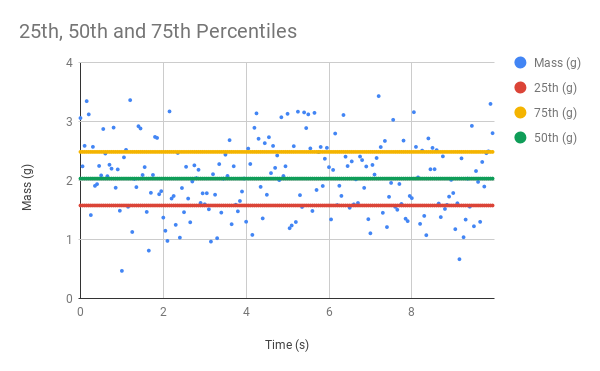
\includegraphics[scale=0.77]{images/00-intro/baseline-quartiles.png}
    \end{center}
    \caption{Quartiles for Baseline Segment}
\end{figure}
%%%%%%%%%%%%%%%%%%%%%%%%%%%%%%%%%%%%%%%%%%%%%%%%%%%%%%%%%%%%%%%%%%%%%%%%%%%%%%%%
\begin{figure} \label{figure.baseline.center}
    \begin{center}
        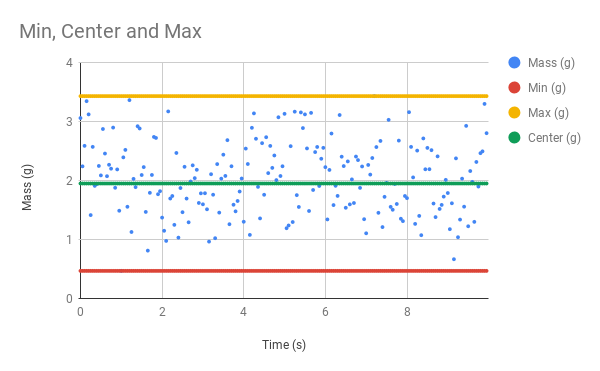
\includegraphics[scale=0.77]{images/00-intro/baseline-min-center-max.png}
    \end{center}
    \caption{Range and Center for Baseline Segment}
\end{figure}
%%%%%%%%%%%%%%%%%%%%%%%%%%%%%%%%%%%%%%%%%%%%%%%%%%%%%%%%%%%%%%%%%%%%%%%%%%%%%%%%
\begin{figure} \label{figure.baseline.chebyshev.1}
    \begin{center}
        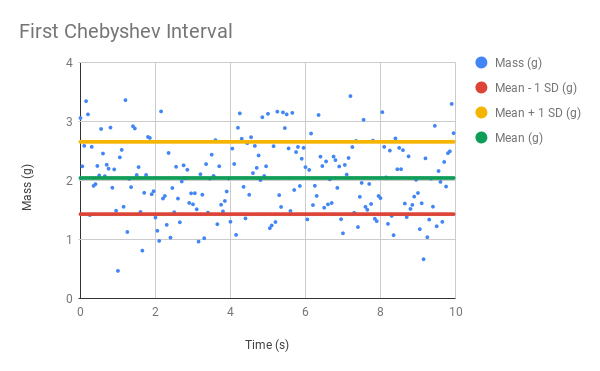
\includegraphics[scale=0.77]{images/00-intro/baseline-chebyshev-1.png}
    \end{center}
    \caption{First Chebyshev Interval for Baseline Segment}
\end{figure}
%%%%%%%%%%%%%%%%%%%%%%%%%%%%%%%%%%%%%%%%%%%%%%%%%%%%%%%%%%%%%%%%%%%%%%%%%%%%%%%%
\begin{figure} \label{figure.baseline.chebyshev.2}
    \begin{center}
        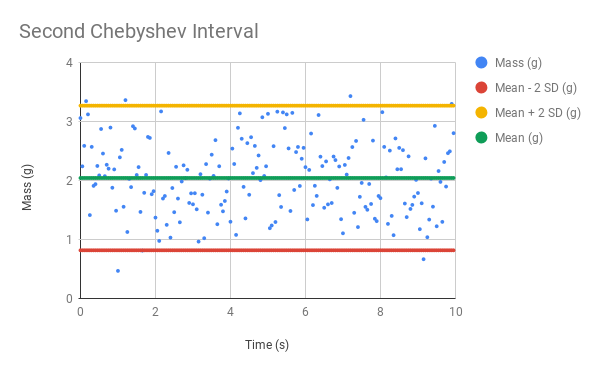
\includegraphics[scale=0.77]{images/00-intro/baseline-chebyshev-2.png}
    \end{center}
    \caption{Second Chebyshev Interval for Baseline Segment}
\end{figure}
%%%%%%%%%%%%%%%%%%%%%%%%%%%%%%%%%%%%%%%%%%%%%%%%%%%%%%%%%%%%%%%%%%%%%%%%%%%%%%%%
\begin{figure} \label{figure.baseline.chebyshev.3}
    \begin{center}
        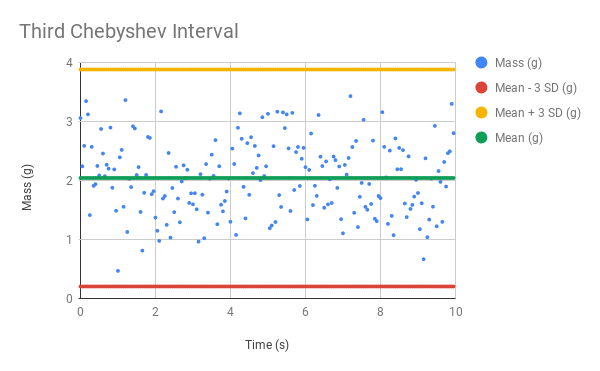
\includegraphics[scale=0.77]{images/00-intro/baseline-chebyshev-3.png}
    \end{center}
    \caption{Third Chebyshev Interval for Baseline Segment}
\end{figure}
%%%%%%%%%%%%%%%%%%%%%%%%%%%%%%%%%%%%%%%%%%%%%%%%%%%%%%%%%%%%%%%%%%%%%%%%%%%%%%%%
\begin{figure} \label{figure.baseline.interval}
    \begin{center}
        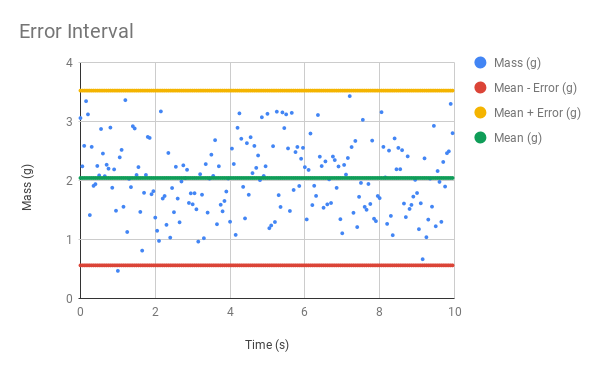
\includegraphics[scale=0.77]{images/00-intro/baseline-error-interval.png}
    \end{center}
    \caption{Error Interval for Baseline Segment}
\end{figure}
%%%%%%%%%%%%%%%%%%%%%%%%%%%%%%%%%%%%%%%%%%%%%%%%%%%%%%%%%%%%%%%%%%%%%%%%%%%%%%%%
\section{Your Data}
%%%%%%%%%%%%%%%%%%%%%%%%%%%%%%%%%%%%%%%%%%%%%%%%%%%%%%%%%%%%%%%%%%%%%%%%%%%%%%%%
Your data also consist of two files:
\begin{itemize}
    \item \texttt{mass.tsv}
    \item \texttt{velocity.tsv}
\end{itemize}
However, the ``theoretical'' values for each section are different. See Table \ref{table.theoretical.v01} and Table \ref{table.theoretical.v02} for specific details.
%%%%%%%%%%%%%%%%%%%%%%%%%%%%%%%%%%%%%%%%%%%%%%%%%%%%%%%%%%%%%%%%%%%%%%%%%%%%%%%%
\begin{table} \label{table.theoretical.v01}
    \centering
    \begin{tabular}{|l|r|}
        \hline
        \textbf{Name} & \textbf{Value} \\
        \hline
        Baseline Mass & 3 g \\
        Mass 1 & 25 g \\
        Mass 2 & 47 g \\
        Standard Deviation & 0.6 g \\
        \hline
        Slope & 13 m/s$^{2}$ \\
        Intercept & 4 m/s \\
        \hline
    \end{tabular}
    \caption{Theoretical values for section V01}
\end{table}
%%%%%%%%%%%%%%%%%%%%%%%%%%%%%%%%%%%%%%%%%%%%%%%%%%%%%%%%%%%%%%%%%%%%%%%%%%%%%%%%
\begin{table} \label{table.theoretical.v02}
    \centering
    \begin{tabular}{|l|r|}
        \hline
        \textbf{Name} & \textbf{Value} \\
        \hline
        Baseline Mass & 4 g \\
        Mass 1 & 23 g \\
        Mass 2 & 53 g \\
        Standard Deviation & 0.6 g \\
        \hline
        Slope & 9 m/s$^{2}$ \\
        Intercept & 2 m/s \\
        \hline
    \end{tabular}
    \caption{Theoretical values for section V02}
\end{table}
%%%%%%%%%%%%%%%%%%%%%%%%%%%%%%%%%%%%%%%%%%%%%%%%%%%%%%%%%%%%%%%%%%%%%%%%%%%%%%%%
\section{Your Lab Report}
%%%%%%%%%%%%%%%%%%%%%%%%%%%%%%%%%%%%%%%%%%%%%%%%%%%%%%%%%%%%%%%%%%%%%%%%%%%%%%%%
There is no written lab report submission for this activity. However, you have to submit a spreadsheet file with your work, which will be graded. Submissions are done via Canvas.

For part 1, your spreadsheet should include the following:
\begin{enumerate}
    \item ...
\end{enumerate}
For part 2, your spreadsheet should include the following:
\begin{enumerate}
    \item ...
\end{enumerate}
The spreadsheet is due on \textbf{Monday, September 10}.
% Copyright 2018 Melvin Eloy Irizarry-Gelpí
\chapter{Error Analysis}
%%%%%%%%%%%%%%%%%%%%%%%%%%%%%%%%%%%%%%%%%%%%%%%%%%%%%%%%%%%%%%%%%%%%%%%%%%%%%%%%
...
%%%%%%%%%%%%%%%%%%%%%%%%%%%%%%%%%%%%%%%%%%%%%%%%%%%%%%%%%%%%%%%%%%%%%%%%%%%%%%%%
\section{Preliminary}
%%%%%%%%%%%%%%%%%%%%%%%%%%%%%%%%%%%%%%%%%%%%%%%%%%%%%%%%%%%%%%%%%%%%%%%%%%%%%%%%
...
%%%%%%%%%%%%%%%%%%%%%%%%%%%%%%%%%%%%%%%%%%%%%%%%%%%%%%%%%%%%%%%%%%%%%%%%%%%%%%%%
\section{Experiment}
%%%%%%%%%%%%%%%%%%%%%%%%%%%%%%%%%%%%%%%%%%%%%%%%%%%%%%%%%%%%%%%%%%%%%%%%%%%%%%%%
...
%%%%%%%%%%%%%%%%%%%%%%%%%%%%%%%%%%%%%%%%%%%%%%%%%%%%%%%%%%%%%%%%%%%%%%%%%%%%%%%%
\section{Analysis}
%%%%%%%%%%%%%%%%%%%%%%%%%%%%%%%%%%%%%%%%%%%%%%%%%%%%%%%%%%%%%%%%%%%%%%%%%%%%%%%%
...
%%%%%%%%%%%%%%%%%%%%%%%%%%%%%%%%%%%%%%%%%%%%%%%%%%%%%%%%%%%%%%%%%%%%%%%%%%%%%%%%
\section{My Data}
%%%%%%%%%%%%%%%%%%%%%%%%%%%%%%%%%%%%%%%%%%%%%%%%%%%%%%%%%%%%%%%%%%%%%%%%%%%%%%%%
...
%%%%%%%%%%%%%%%%%%%%%%%%%%%%%%%%%%%%%%%%%%%%%%%%%%%%%%%%%%%%%%%%%%%%%%%%%%%%%%%%
\section{Your Data}
%%%%%%%%%%%%%%%%%%%%%%%%%%%%%%%%%%%%%%%%%%%%%%%%%%%%%%%%%%%%%%%%%%%%%%%%%%%%%%%%
...
%%%%%%%%%%%%%%%%%%%%%%%%%%%%%%%%%%%%%%%%%%%%%%%%%%%%%%%%%%%%%%%%%%%%%%%%%%%%%%%%
\section{Your Lab Report}
%%%%%%%%%%%%%%%%%%%%%%%%%%%%%%%%%%%%%%%%%%%%%%%%%%%%%%%%%%%%%%%%%%%%%%%%%%%%%%%%
...
% Copyright 2018 Melvin Eloy Irizarry-Gelpí
\chapter{Motion on an Incline}
%%%%%%%%%%%%%%%%%%%%%%%%%%%%%%%%%%%%%%%%%%%%%%%%%%%%%%%%%%%%%%%%%%%%%%%%%%%%%%%%
...
%%%%%%%%%%%%%%%%%%%%%%%%%%%%%%%%%%%%%%%%%%%%%%%%%%%%%%%%%%%%%%%%%%%%%%%%%%%%%%%%
\section{Preliminary}
%%%%%%%%%%%%%%%%%%%%%%%%%%%%%%%%%%%%%%%%%%%%%%%%%%%%%%%%%%%%%%%%%%%%%%%%%%%%%%%%
...
%%%%%%%%%%%%%%%%%%%%%%%%%%%%%%%%%%%%%%%%%%%%%%%%%%%%%%%%%%%%%%%%%%%%%%%%%%%%%%%%
\section{Experiment}
%%%%%%%%%%%%%%%%%%%%%%%%%%%%%%%%%%%%%%%%%%%%%%%%%%%%%%%%%%%%%%%%%%%%%%%%%%%%%%%%
...
%%%%%%%%%%%%%%%%%%%%%%%%%%%%%%%%%%%%%%%%%%%%%%%%%%%%%%%%%%%%%%%%%%%%%%%%%%%%%%%%
\section{Analysis}
%%%%%%%%%%%%%%%%%%%%%%%%%%%%%%%%%%%%%%%%%%%%%%%%%%%%%%%%%%%%%%%%%%%%%%%%%%%%%%%%
...
%%%%%%%%%%%%%%%%%%%%%%%%%%%%%%%%%%%%%%%%%%%%%%%%%%%%%%%%%%%%%%%%%%%%%%%%%%%%%%%%
\section{My Data}
%%%%%%%%%%%%%%%%%%%%%%%%%%%%%%%%%%%%%%%%%%%%%%%%%%%%%%%%%%%%%%%%%%%%%%%%%%%%%%%%
...
%%%%%%%%%%%%%%%%%%%%%%%%%%%%%%%%%%%%%%%%%%%%%%%%%%%%%%%%%%%%%%%%%%%%%%%%%%%%%%%%
\section{Your Data}
%%%%%%%%%%%%%%%%%%%%%%%%%%%%%%%%%%%%%%%%%%%%%%%%%%%%%%%%%%%%%%%%%%%%%%%%%%%%%%%%
...
%%%%%%%%%%%%%%%%%%%%%%%%%%%%%%%%%%%%%%%%%%%%%%%%%%%%%%%%%%%%%%%%%%%%%%%%%%%%%%%%
\section{Your Lab Report}
%%%%%%%%%%%%%%%%%%%%%%%%%%%%%%%%%%%%%%%%%%%%%%%%%%%%%%%%%%%%%%%%%%%%%%%%%%%%%%%%
...
\chapter{Newton's First Law}
%%%%%%%%%%%%%%%%%%%%%%%%%%%%%%%%%%%%%%%%%%%%%%%%%%%%%%%%%%%%%%%%%%%%%%%%%%%%%%%%%%%%%%%%%
...
%%%%%%%%%%%%%%%%%%%%%%%%%%%%%%%%%%%%%%%%%%%%%%%%%%%%%%%%%%%%%%%%%%%%%%%%%%%%%%%%%%%%%%%%%
\section{Preliminary}
%%%%%%%%%%%%%%%%%%%%%%%%%%%%%%%%%%%%%%%%%%%%%%%%%%%%%%%%%%%%%%%%%%%%%%%%%%%%%%%%%%%%%%%%%
...
%%%%%%%%%%%%%%%%%%%%%%%%%%%%%%%%%%%%%%%%%%%%%%%%%%%%%%%%%%%%%%%%%%%%%%%%%%%%%%%%%%%%%%%%%
\section{Experiment}
%%%%%%%%%%%%%%%%%%%%%%%%%%%%%%%%%%%%%%%%%%%%%%%%%%%%%%%%%%%%%%%%%%%%%%%%%%%%%%%%%%%%%%%%%
...
%%%%%%%%%%%%%%%%%%%%%%%%%%%%%%%%%%%%%%%%%%%%%%%%%%%%%%%%%%%%%%%%%%%%%%%%%%%%%%%%%%%%%%%%%
\section{Analysis}
%%%%%%%%%%%%%%%%%%%%%%%%%%%%%%%%%%%%%%%%%%%%%%%%%%%%%%%%%%%%%%%%%%%%%%%%%%%%%%%%%%%%%%%%%
...
%%%%%%%%%%%%%%%%%%%%%%%%%%%%%%%%%%%%%%%%%%%%%%%%%%%%%%%%%%%%%%%%%%%%%%%%%%%%%%%%%%%%%%%%%
\section{My Data}
%%%%%%%%%%%%%%%%%%%%%%%%%%%%%%%%%%%%%%%%%%%%%%%%%%%%%%%%%%%%%%%%%%%%%%%%%%%%%%%%%%%%%%%%%
...
%%%%%%%%%%%%%%%%%%%%%%%%%%%%%%%%%%%%%%%%%%%%%%%%%%%%%%%%%%%%%%%%%%%%%%%%%%%%%%%%%%%%%%%%%
\section{Your Data}
%%%%%%%%%%%%%%%%%%%%%%%%%%%%%%%%%%%%%%%%%%%%%%%%%%%%%%%%%%%%%%%%%%%%%%%%%%%%%%%%%%%%%%%%%
...
%%%%%%%%%%%%%%%%%%%%%%%%%%%%%%%%%%%%%%%%%%%%%%%%%%%%%%%%%%%%%%%%%%%%%%%%%%%%%%%%%%%%%%%%%
\section{Your Lab Report}
%%%%%%%%%%%%%%%%%%%%%%%%%%%%%%%%%%%%%%%%%%%%%%%%%%%%%%%%%%%%%%%%%%%%%%%%%%%%%%%%%%%%%%%%%
...
% Copyright 2018 Melvin Eloy Irizarry-Gelpí
\chapter{Newton's Second Law}
%%%%%%%%%%%%%%%%%%%%%%%%%%%%%%%%%%%%%%%%%%%%%%%%%%%%%%%%%%%%%%%%%%%%%%%%%%%%%%%%
...
%%%%%%%%%%%%%%%%%%%%%%%%%%%%%%%%%%%%%%%%%%%%%%%%%%%%%%%%%%%%%%%%%%%%%%%%%%%%%%%%
\section{Preliminary}
%%%%%%%%%%%%%%%%%%%%%%%%%%%%%%%%%%%%%%%%%%%%%%%%%%%%%%%%%%%%%%%%%%%%%%%%%%%%%%%%
...
%%%%%%%%%%%%%%%%%%%%%%%%%%%%%%%%%%%%%%%%%%%%%%%%%%%%%%%%%%%%%%%%%%%%%%%%%%%%%%%%
\section{Experiment}
%%%%%%%%%%%%%%%%%%%%%%%%%%%%%%%%%%%%%%%%%%%%%%%%%%%%%%%%%%%%%%%%%%%%%%%%%%%%%%%%
...
%%%%%%%%%%%%%%%%%%%%%%%%%%%%%%%%%%%%%%%%%%%%%%%%%%%%%%%%%%%%%%%%%%%%%%%%%%%%%%%%
\section{Analysis}
%%%%%%%%%%%%%%%%%%%%%%%%%%%%%%%%%%%%%%%%%%%%%%%%%%%%%%%%%%%%%%%%%%%%%%%%%%%%%%%%
...
%%%%%%%%%%%%%%%%%%%%%%%%%%%%%%%%%%%%%%%%%%%%%%%%%%%%%%%%%%%%%%%%%%%%%%%%%%%%%%%%
\section{My Data}
%%%%%%%%%%%%%%%%%%%%%%%%%%%%%%%%%%%%%%%%%%%%%%%%%%%%%%%%%%%%%%%%%%%%%%%%%%%%%%%%
...
%%%%%%%%%%%%%%%%%%%%%%%%%%%%%%%%%%%%%%%%%%%%%%%%%%%%%%%%%%%%%%%%%%%%%%%%%%%%%%%%
\section{Your Data}
%%%%%%%%%%%%%%%%%%%%%%%%%%%%%%%%%%%%%%%%%%%%%%%%%%%%%%%%%%%%%%%%%%%%%%%%%%%%%%%%
...
%%%%%%%%%%%%%%%%%%%%%%%%%%%%%%%%%%%%%%%%%%%%%%%%%%%%%%%%%%%%%%%%%%%%%%%%%%%%%%%%
\section{Your Lab Report}
%%%%%%%%%%%%%%%%%%%%%%%%%%%%%%%%%%%%%%%%%%%%%%%%%%%%%%%%%%%%%%%%%%%%%%%%%%%%%%%%
...
\chapter{Newton's Third Law}
%%%%%%%%%%%%%%%%%%%%%%%%%%%%%%%%%%%%%%%%%%%%%%%%%%%%%%%%%%%%%%%%%%%%%%%%%%%%%%%%%%%%%%%%%
...
%%%%%%%%%%%%%%%%%%%%%%%%%%%%%%%%%%%%%%%%%%%%%%%%%%%%%%%%%%%%%%%%%%%%%%%%%%%%%%%%%%%%%%%%%
\section{Preliminary}
%%%%%%%%%%%%%%%%%%%%%%%%%%%%%%%%%%%%%%%%%%%%%%%%%%%%%%%%%%%%%%%%%%%%%%%%%%%%%%%%%%%%%%%%%
...
%%%%%%%%%%%%%%%%%%%%%%%%%%%%%%%%%%%%%%%%%%%%%%%%%%%%%%%%%%%%%%%%%%%%%%%%%%%%%%%%%%%%%%%%%
\section{Experiment}
%%%%%%%%%%%%%%%%%%%%%%%%%%%%%%%%%%%%%%%%%%%%%%%%%%%%%%%%%%%%%%%%%%%%%%%%%%%%%%%%%%%%%%%%%
...
%%%%%%%%%%%%%%%%%%%%%%%%%%%%%%%%%%%%%%%%%%%%%%%%%%%%%%%%%%%%%%%%%%%%%%%%%%%%%%%%%%%%%%%%%
\section{Analysis}
%%%%%%%%%%%%%%%%%%%%%%%%%%%%%%%%%%%%%%%%%%%%%%%%%%%%%%%%%%%%%%%%%%%%%%%%%%%%%%%%%%%%%%%%%
...
%%%%%%%%%%%%%%%%%%%%%%%%%%%%%%%%%%%%%%%%%%%%%%%%%%%%%%%%%%%%%%%%%%%%%%%%%%%%%%%%%%%%%%%%%
\section{My Data}
%%%%%%%%%%%%%%%%%%%%%%%%%%%%%%%%%%%%%%%%%%%%%%%%%%%%%%%%%%%%%%%%%%%%%%%%%%%%%%%%%%%%%%%%%
...
%%%%%%%%%%%%%%%%%%%%%%%%%%%%%%%%%%%%%%%%%%%%%%%%%%%%%%%%%%%%%%%%%%%%%%%%%%%%%%%%%%%%%%%%%
\section{Your Data}
%%%%%%%%%%%%%%%%%%%%%%%%%%%%%%%%%%%%%%%%%%%%%%%%%%%%%%%%%%%%%%%%%%%%%%%%%%%%%%%%%%%%%%%%%
...
%%%%%%%%%%%%%%%%%%%%%%%%%%%%%%%%%%%%%%%%%%%%%%%%%%%%%%%%%%%%%%%%%%%%%%%%%%%%%%%%%%%%%%%%%
\section{Your Lab Report}
%%%%%%%%%%%%%%%%%%%%%%%%%%%%%%%%%%%%%%%%%%%%%%%%%%%%%%%%%%%%%%%%%%%%%%%%%%%%%%%%%%%%%%%%%
...
\chapter{Kinetic Energy}
%%%%%%%%%%%%%%%%%%%%%%%%%%%%%%%%%%%%%%%%%%%%%%%%%%%%%%%%%%%%%%%%%%%%%%%%%%%%%%%%%%%%%%%%%
...
%%%%%%%%%%%%%%%%%%%%%%%%%%%%%%%%%%%%%%%%%%%%%%%%%%%%%%%%%%%%%%%%%%%%%%%%%%%%%%%%%%%%%%%%%
\section{Preliminary}
%%%%%%%%%%%%%%%%%%%%%%%%%%%%%%%%%%%%%%%%%%%%%%%%%%%%%%%%%%%%%%%%%%%%%%%%%%%%%%%%%%%%%%%%%
...
%%%%%%%%%%%%%%%%%%%%%%%%%%%%%%%%%%%%%%%%%%%%%%%%%%%%%%%%%%%%%%%%%%%%%%%%%%%%%%%%%%%%%%%%%
\section{Experiment}
%%%%%%%%%%%%%%%%%%%%%%%%%%%%%%%%%%%%%%%%%%%%%%%%%%%%%%%%%%%%%%%%%%%%%%%%%%%%%%%%%%%%%%%%%
...
%%%%%%%%%%%%%%%%%%%%%%%%%%%%%%%%%%%%%%%%%%%%%%%%%%%%%%%%%%%%%%%%%%%%%%%%%%%%%%%%%%%%%%%%%
\section{Analysis}
%%%%%%%%%%%%%%%%%%%%%%%%%%%%%%%%%%%%%%%%%%%%%%%%%%%%%%%%%%%%%%%%%%%%%%%%%%%%%%%%%%%%%%%%%
...
%%%%%%%%%%%%%%%%%%%%%%%%%%%%%%%%%%%%%%%%%%%%%%%%%%%%%%%%%%%%%%%%%%%%%%%%%%%%%%%%%%%%%%%%%
\section{My Data}
%%%%%%%%%%%%%%%%%%%%%%%%%%%%%%%%%%%%%%%%%%%%%%%%%%%%%%%%%%%%%%%%%%%%%%%%%%%%%%%%%%%%%%%%%
...
%%%%%%%%%%%%%%%%%%%%%%%%%%%%%%%%%%%%%%%%%%%%%%%%%%%%%%%%%%%%%%%%%%%%%%%%%%%%%%%%%%%%%%%%%
\section{Your Data}
%%%%%%%%%%%%%%%%%%%%%%%%%%%%%%%%%%%%%%%%%%%%%%%%%%%%%%%%%%%%%%%%%%%%%%%%%%%%%%%%%%%%%%%%%
...
%%%%%%%%%%%%%%%%%%%%%%%%%%%%%%%%%%%%%%%%%%%%%%%%%%%%%%%%%%%%%%%%%%%%%%%%%%%%%%%%%%%%%%%%%
\section{Your Lab Report}
%%%%%%%%%%%%%%%%%%%%%%%%%%%%%%%%%%%%%%%%%%%%%%%%%%%%%%%%%%%%%%%%%%%%%%%%%%%%%%%%%%%%%%%%%
...
% Copyright 2018 Melvin Eloy Irizarry-Gelpí
\chapter{Mechanic Energy}
%%%%%%%%%%%%%%%%%%%%%%%%%%%%%%%%%%%%%%%%%%%%%%%%%%%%%%%%%%%%%%%%%%%%%%%%%%%%%%%%
...
%%%%%%%%%%%%%%%%%%%%%%%%%%%%%%%%%%%%%%%%%%%%%%%%%%%%%%%%%%%%%%%%%%%%%%%%%%%%%%%%
\section{Preliminary}
%%%%%%%%%%%%%%%%%%%%%%%%%%%%%%%%%%%%%%%%%%%%%%%%%%%%%%%%%%%%%%%%%%%%%%%%%%%%%%%%
There are many kinds of energy. You have \textbf{kinetic energy}, which is associated with motion. The amount of kinetic energy $K$ depends on the amount of mass $m$ and the amount of speed $v$:
\begin{equation}
    K = \frac{1}{2} m v^{2}
\end{equation}
Note that kinetic energy changes if the velocity of the object changes.

You have \textbf{gravitational energy} (a form of potential energy), which is associated to being in a region with a gravitational field. The amount of gravitational energy $U_{g}$ depends on the amount of mass $m$, the amount of gravitational acceleration $g$, and the amount of height $h$ measured from a reference point:
\begin{equation}
    U_{g} = m g h
\end{equation}
Note that the gravitational energy changes if the height of the object changes.

Finally, you have \textbf{mechanic energy}. The amount of mechanic energy $E$ is just the sum of kinetic energy $K$ and potential energy. In the case when the potential energy is only gravitational in nature, then the mechanic energy is
\begin{equation}
    E = K + U_{g}
\end{equation}
Energy cannot be created nor destroyed; it can only be transformed into other forms of energy. In a closed system, where energy is not added nor removed by an external source, mechanic energy $E$ is \textbf{constant in time}.

If the object only moves and feels gravity, then the mechanic energy $E$ is given by
\begin{equation}
    E = \frac{1}{2} m v^{2} + m g h
\end{equation}
Solving for $v^{2}$ you get
\begin{equation}
    v^{2} = \left( - 2 g \right) h + \left( \frac{2 E}{m} \right)
    \label{eq.07.vv}
\end{equation}
This relation predicts that $v^{2}$ is a \textbf{linear function} of $h$ with the slope being $-2g$ and the intercept being $2 E / m$. That is, the data in a $v^{2}$ versus $h$ graph should have a \textbf{linear shape}.
%%%%%%%%%%%%%%%%%%%%%%%%%%%%%%%%%%%%%%%%%%%%%%%%%%%%%%%%%%%%%%%%%%%%%%%%%%%%%%%%
\section{Experiment}
%%%%%%%%%%%%%%%%%%%%%%%%%%%%%%%%%%%%%%%%%%%%%%%%%%%%%%%%%%%%%%%%%%%%%%%%%%%%%%%%
In order to study a system where there is gravitational energy, and also that that gravitational changes with time, we used an object moving along an incline. With a motion sensor, we recorded the \textbf{position} $d$ and \textbf{velocity} $v$ along the incline as they changed with time. You also recorded some height measurements to determine the sine of the angle of inclination $\theta$ of the incline. Also, you recorded the mass $m$ of the cart.
%%%%%%%%%%%%%%%%%%%%%%%%%%%%%%%%%%%%%%%%%%%%%%%%%%%%%%%%%%%%%%%%%%%%%%%%%%%%%%%%
\section{Analysis}
%%%%%%%%%%%%%%%%%%%%%%%%%%%%%%%%%%%%%%%%%%%%%%%%%%%%%%%%%%%%%%%%%%%%%%%%%%%%%%%%
We would like to test two predictions:
\begin{enumerate}
    \item Mechanic energy does not change with time.
    \item There is a linear relation between $v^{2}$ and $h$ given by equation (\ref{eq.07.vv}).
\end{enumerate}
To test the first prediction, we need to compute the mechanic energy with the data that we collected. To test the second prediction, we need to make a graph with $v^{2}$ in the vertical axis and $h$ in the horizontal axis.

Here are some steps to complete the analysis.
%%%%%%%%%%%%%%%%%%%%%%%%%%%%%%%%%%%%%%%%%%%%%%%%%%%%%%%%%%%%%%%%%%%%%%%%%%%%%%%%
\subsection{Calculate Sine}
%%%%%%%%%%%%%%%%%%%%%%%%%%%%%%%%%%%%%%%%%%%%%%%%%%%%%%%%%%%%%%%%%%%%%%%%%%%%%%%%
You measured the heights of four positions along the incline:
\begin{equation}
    h_{1} \qquad h_{2} \qquad h_{3} \qquad h_{4}
\end{equation}
Assuming that the four positions are equally separated by a distance $x$ (I used 10 cm; some people used that also; others did 20 cm), then the sine of the angle should be given by the following three calculations:
\begin{equation}
    \sin{(\theta_{1})} = \frac{h_{2} - h_{1}}{x}, \qquad \sin{(\theta_{2})} = \frac{h_{3} - h_{2}}{x}, \qquad \sin{(\theta_{3})} = \frac{h_{4} - h_{3}}{x}
\end{equation}
You can think of each of these as an independent measurement, so take the average value of the three and use that as the value for the sine of the angle:
\begin{equation}
    \sin{(\theta)} = \frac{1}{3} \left[ \sin{(\theta_{1})} + \sin{(\theta_{2})} + \sin{(\theta_{3})} \right]
\end{equation}
You need this sine because the height $h$ at the incline is related to the position $d$ along the incline by the relation
\begin{equation}
    h = d \sin{(\theta)}
\end{equation}
%%%%%%%%%%%%%%%%%%%%%%%%%%%%%%%%%%%%%%%%%%%%%%%%%%%%%%%%%%%%%%%%%%%%%%%%%%%%%%%%
\subsection{Truncate the Data}
%%%%%%%%%%%%%%%%%%%%%%%%%%%%%%%%%%%%%%%%%%%%%%%%%%%%%%%%%%%%%%%%%%%%%%%%%%%%%%%%
Before you can do anything with the data from the experiment, you need to isolated the part of the data where the motion along the incline is happening. In order to know where to cut the data, it is best to make a scatter plot with velocity in the vertical axis and time in the horizontal axis. There are three kinds of truncation:
\begin{enumerate}
    \item Upward motion only: find the time just after the velocity values begin the diagonal downward trend, and the time when the velocity is close to zero
    \item Downward motion only: find the time when the velocity is close to zero, and the time just before the velocity ends the diagonal downward trend
    \item Upward and downward motion: find the time just after the velocity values begin the diagonal downward trend, and the time just before the downward trend ends
\end{enumerate}
Once you know the initial time and the final time of the motion, just delete the data outside of this time interval.
%%%%%%%%%%%%%%%%%%%%%%%%%%%%%%%%%%%%%%%%%%%%%%%%%%%%%%%%%%%%%%%%%%%%%%%%%%%%%%%%
\subsection{Calculate Height}
%%%%%%%%%%%%%%%%%%%%%%%%%%%%%%%%%%%%%%%%%%%%%%%%%%%%%%%%%%%%%%%%%%%%%%%%%%%%%%%%
In a separate column, you should compute the value of the height on the incline using the values in the position column. If $d$ is a position value, then the corresponding height is given by
\begin{equation}
    h = d \sin{(\theta)}
\end{equation}
%%%%%%%%%%%%%%%%%%%%%%%%%%%%%%%%%%%%%%%%%%%%%%%%%%%%%%%%%%%%%%%%%%%%%%%%%%%%%%%%
\subsection{Calculate Kinetic Energy}
%%%%%%%%%%%%%%%%%%%%%%%%%%%%%%%%%%%%%%%%%%%%%%%%%%%%%%%%%%%%%%%%%%%%%%%%%%%%%%%%
In a separate column, you should compute the value of the kinetic energy using the values in the velocity column. If $v$ is a velocity value, then the corresponding kinetic energy is given by
\begin{equation}
    K = \frac{1}{2} m v^{2}
\end{equation}
%%%%%%%%%%%%%%%%%%%%%%%%%%%%%%%%%%%%%%%%%%%%%%%%%%%%%%%%%%%%%%%%%%%%%%%%%%%%%%%%
\subsection{Calculate Gravitational Energy}
%%%%%%%%%%%%%%%%%%%%%%%%%%%%%%%%%%%%%%%%%%%%%%%%%%%%%%%%%%%%%%%%%%%%%%%%%%%%%%%%
In a separate column, you should compute the value of the gravitational energy using the values in the height column. If $h$ is a height value, then the corresponding gravitational energy is given by
\begin{equation}
    U_{g} = m g h
\end{equation}
%%%%%%%%%%%%%%%%%%%%%%%%%%%%%%%%%%%%%%%%%%%%%%%%%%%%%%%%%%%%%%%%%%%%%%%%%%%%%%%%
\subsection{Calculate Mechanic Energy}
%%%%%%%%%%%%%%%%%%%%%%%%%%%%%%%%%%%%%%%%%%%%%%%%%%%%%%%%%%%%%%%%%%%%%%%%%%%%%%%%
In a separate column, you should compute the value of the mechanic energy using the values in the kinetic and gravitational energy columns. If $K$ is a value in the kinetic energy column, and $U_{g}$ is a value in the gravitational energy column, then the mechanic energy is given by
\begin{equation}
    E = K + U_{g}
\end{equation}
Make sure that you add values that are evaluated at the same time.
%%%%%%%%%%%%%%%%%%%%%%%%%%%%%%%%%%%%%%%%%%%%%%%%%%%%%%%%%%%%%%%%%%%%%%%%%%%%%%%%
\subsection{Graph Mechanic Energy vs Time}
%%%%%%%%%%%%%%%%%%%%%%%%%%%%%%%%%%%%%%%%%%%%%%%%%%%%%%%%%%%%%%%%%%%%%%%%%%%%%%%%
One of the goals of this experiment is to verify that mechanic energy is constant in time. To check this, you can make a scatter plot with time in the horizontal axis and mechanic energy in the vertical axis. In principle, you should see that the values of mechanic energy do not change with time. In practice, we see that in general the mechanic energy decreases as time passes. This is actually true, since in this experiment we could not completely remove friction and this force leads to a dissipation of energy. However, the amount of change in energy over time is very small, so effectively and approximately mechanic energy is constant.

In particular, note that the energy values in my run 6 (figure \ref{figure.07.run.6.e}) appear to be random. This strongly suggest that the variations are more related to noise than anything physical.
%%%%%%%%%%%%%%%%%%%%%%%%%%%%%%%%%%%%%%%%%%%%%%%%%%%%%%%%%%%%%%%%%%%%%%%%%%%%%%%%
\begin{figure}
    \begin{center}
	    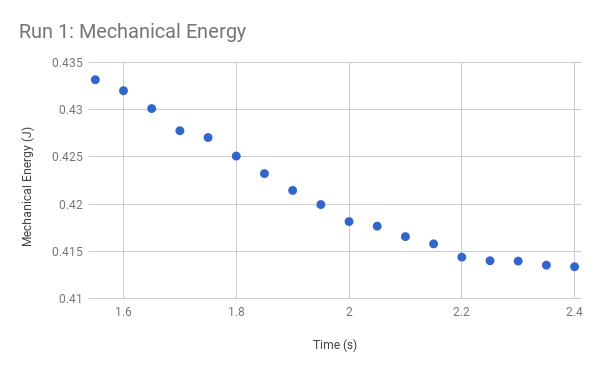
\includegraphics[scale=0.77]{images/07-mechanic/run-1-energy.png}
    \end{center}
    \caption{}
    \label{figure.07.run.1.e}
\end{figure}
%%%%%%%%%%%%%%%%%%%%%%%%%%%%%%%%%%%%%%%%%%%%%%%%%%%%%%%%%%%%%%%%%%%%%%%%%%%%%%%%
\begin{figure}
    \begin{center}
	    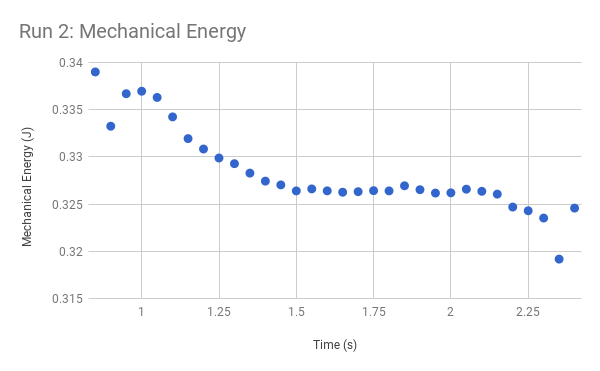
\includegraphics[scale=0.77]{images/07-mechanic/run-2-energy.png}
    \end{center}
    \caption{}
    \label{figure.07.run.2.e}
\end{figure}
%%%%%%%%%%%%%%%%%%%%%%%%%%%%%%%%%%%%%%%%%%%%%%%%%%%%%%%%%%%%%%%%%%%%%%%%%%%%%%%%
\begin{figure}
    \begin{center}
	    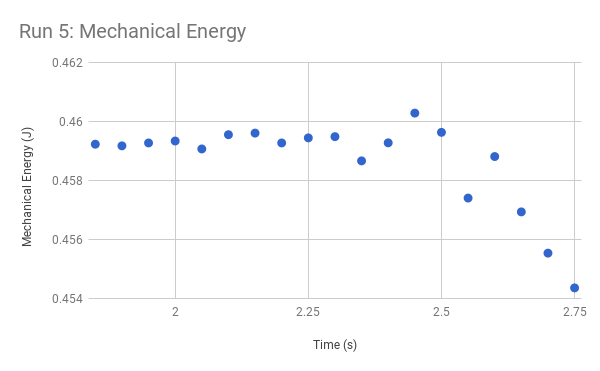
\includegraphics[scale=0.77]{images/07-mechanic/run-5-energy.png}
    \end{center}
    \caption{}
    \label{figure.07.run.5.e}
\end{figure}
%%%%%%%%%%%%%%%%%%%%%%%%%%%%%%%%%%%%%%%%%%%%%%%%%%%%%%%%%%%%%%%%%%%%%%%%%%%%%%%%
\begin{figure}
    \begin{center}
	    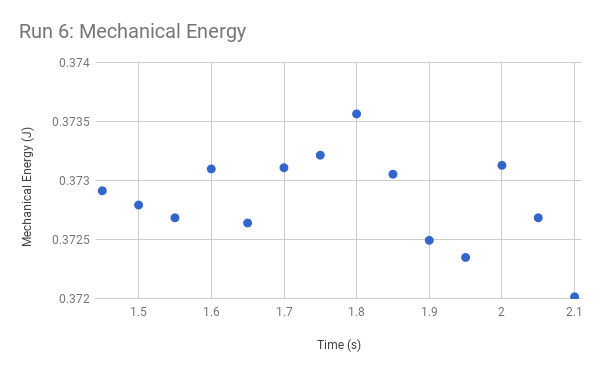
\includegraphics[scale=0.77]{images/07-mechanic/run-6-energy.png}
    \end{center}
    \caption{}
    \label{figure.07.run.6.e}
\end{figure}
%%%%%%%%%%%%%%%%%%%%%%%%%%%%%%%%%%%%%%%%%%%%%%%%%%%%%%%%%%%%%%%%%%%%%%%%%%%%%%%%
\subsection{Calculate Velocity Squared}
%%%%%%%%%%%%%%%%%%%%%%%%%%%%%%%%%%%%%%%%%%%%%%%%%%%%%%%%%%%%%%%%%%%%%%%%%%%%%%%%
In a separate column, you should calculate the velocity squared using the values in the velocity column. If $v$ is a velocity values, then the velocity square is $v^2$ or equivalently $v \times v$.
%%%%%%%%%%%%%%%%%%%%%%%%%%%%%%%%%%%%%%%%%%%%%%%%%%%%%%%%%%%%%%%%%%%%%%%%%%%%%%%%
\subsection{Graph $v^2$ vs $h$}
%%%%%%%%%%%%%%%%%%%%%%%%%%%%%%%%%%%%%%%%%%%%%%%%%%%%%%%%%%%%%%%%%%%%%%%%%%%%%%%%
The other goal of this experiment was to verify the linear relation between $v^{2}$ and $h$ suggested by equation (\ref{eq.07.vv}) due to conservation of energy. Since the relation is a linear function, the data points should arrange themselves to form a linear shape. You can use Google Sheets or Excel to find the best linear fit. In Google Sheets, this is under ``Series'' in the chart editor. You need to check the ``Trend line'' box and make sure that it is ``Linear''. It is good practice to reduce the size of the data points (I use 2px) and to use a color for the trend line that is different from the color of the data points. In my case I have blue data points for the experimental data and red line for the best fit line.

If the data were perfect, then the slope of this linear fit should be given by
\begin{equation}
    \text{slope } = -2g = 19.6 \text{ m/s}^{2}
    \label{eq.07.slope}
\end{equation}
and the intercept would be related to the amount of mechanic energy via
\begin{equation}
    \text{intercept } = \frac{2 E}{m}
\end{equation}
The slope is negative, so we should see a diagonal line that is downward as height increases. From the intercept you can get a value for mechanic energy that should be close to what you found in the mechanic energy column:
\begin{equation}
    E = \frac{m \times \text{ intercept}}{2}
    \label{eq.07.intercept}
\end{equation}
You can also compare this value with the average of the mechanic energy column (use the \texttt{AVERAGE} function to compute this). Note that this is an average over time.
%%%%%%%%%%%%%%%%%%%%%%%%%%%%%%%%%%%%%%%%%%%%%%%%%%%%%%%%%%%%%%%%%%%%%%%%%%%%%%%%
\begin{figure}
    \begin{center}
	    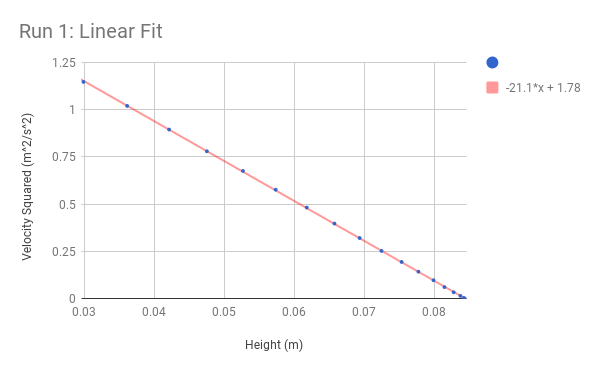
\includegraphics[scale=0.77]{images/07-mechanic/run-1-fit.png}
    \end{center}
    \caption{}
    \label{figure.07.run.1.fit}
\end{figure}
%%%%%%%%%%%%%%%%%%%%%%%%%%%%%%%%%%%%%%%%%%%%%%%%%%%%%%%%%%%%%%%%%%%%%%%%%%%%%%%%
\begin{figure}
    \begin{center}
	    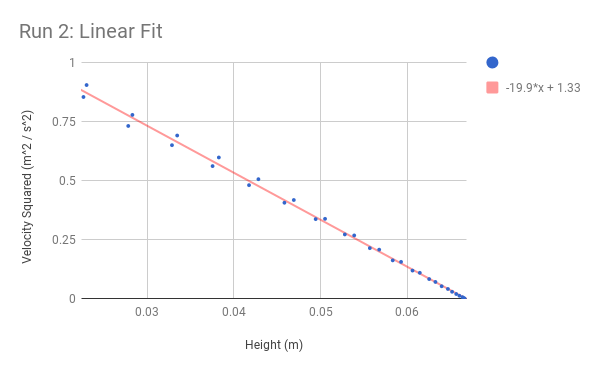
\includegraphics[scale=0.77]{images/07-mechanic/run-2-fit.png}
    \end{center}
    \caption{}
    \label{figure.07.run.2.fit}
\end{figure}
%%%%%%%%%%%%%%%%%%%%%%%%%%%%%%%%%%%%%%%%%%%%%%%%%%%%%%%%%%%%%%%%%%%%%%%%%%%%%%%%
\begin{figure}
    \begin{center}
	    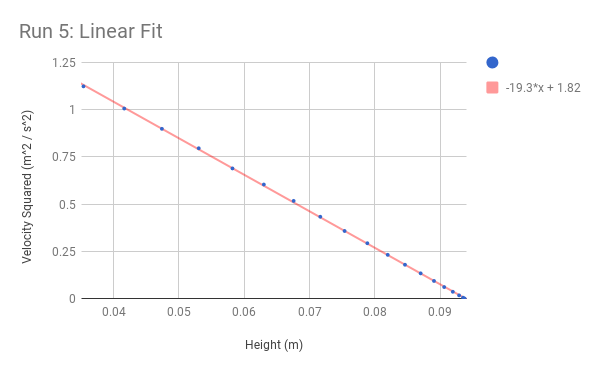
\includegraphics[scale=0.77]{images/07-mechanic/run-5-fit.png}
    \end{center}
    \caption{}
    \label{figure.07.run.5.fit}
\end{figure}
%%%%%%%%%%%%%%%%%%%%%%%%%%%%%%%%%%%%%%%%%%%%%%%%%%%%%%%%%%%%%%%%%%%%%%%%%%%%%%%%
\begin{figure}
    \begin{center}
	    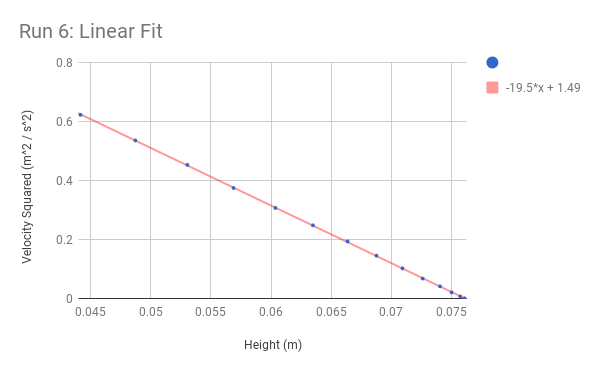
\includegraphics[scale=0.77]{images/07-mechanic/run-6-fit.png}
    \end{center}
    \caption{}
    \label{figure.07.run.6.fit}
\end{figure}
%%%%%%%%%%%%%%%%%%%%%%%%%%%%%%%%%%%%%%%%%%%%%%%%%%%%%%%%%%%%%%%%%%%%%%%%%%%%%%%%
\section{My Data}
%%%%%%%%%%%%%%%%%%%%%%%%%%%%%%%%%%%%%%%%%%%%%%%%%%%%%%%%%%%%%%%%%%%%%%%%%%%%%%%%
I collected ten runs of data. In run 1, I used a truncation that only kept the upward motion. In run 2, I used a truncation that kept the upward and the downward motion. For run 5 and 6, I used a truncation that only kept the downward motion. As you can see, the linear fits are very appropriate, so the data does satisfy a linear relation. Furthermore, the values for the slope agree with the prediction: they are all very close to the predicted value in (\ref{eq.07.slope}). Also, the value of the intercept can be used in equation (\ref{eq.07.intercept}) to obtain an energy value that agrees with the time average mechanic energy.

Let us extract these values from a graph. Look at graph \ref{figure.07.run.6.fit} for run 6. The slope is -19.5 m/s$^{2}$. The intercept is 1.49 m$^{2}$/s$^{2}$. If the mass is 0.5 kg, then
\begin{equation}
    \frac{m \times \text{ intercept}}{2} = \frac{1}{2} (0.5 \text{ kg}) (1.49 \text{ m}^{2}\text{/s}^{2}) = 0.3717 \text{ J}
\end{equation}
This number is close to the time-average of the mechanic energy: 0.3728 J.

Here is a table summarizing some of my results.
%%%%%%%%%%%%%%%%%%%%%%%%%%%%%%%%%%%%%%%%%%%%%%%%%%%%%%%%%%%%%%%%%%%%%%%%%%%%%%%%
\begin{table}
	\begin{center}
		\begin{tabular}{|r|r|r|r|r|}\hline
			Run & 1 & 2 & 5 & 6 \\ \hline
			Slope (m/s$^{2}$) & -21.1 & -19.9 & -19.3 & -19.5 \\
            Intercept (m$^{2}$/s$^{2}$) & 1.78 & 1.33 & 1.82 & 1.49 \\
            $E$ from intercept (J) & 0.4460 & 0.3326 & 0.4540 & 0.3717 \\
            Time-averaged $E$ (J) & 0.4210 & 0.3283 & 0.4587 & 0.3728 \\
			\hline
		\end{tabular}
	\end{center}
	\caption{Summary of results}
	\label{table.07.results}
\end{table}
%%%%%%%%%%%%%%%%%%%%%%%%%%%%%%%%%%%%%%%%%%%%%%%%%%%%%%%%%%%%%%%%%%%%%%%%%%%%%%%%
\section{Your Data}
%%%%%%%%%%%%%%%%%%%%%%%%%%%%%%%%%%%%%%%%%%%%%%%%%%%%%%%%%%%%%%%%%%%%%%%%%%%%%%%%
You should have ten runs of data as well.
%%%%%%%%%%%%%%%%%%%%%%%%%%%%%%%%%%%%%%%%%%%%%%%%%%%%%%%%%%%%%%%%%%%%%%%%%%%%%%%%
\section{Your Lab Report}
%%%%%%%%%%%%%%%%%%%%%%%%%%%%%%%%%%%%%%%%%%%%%%%%%%%%%%%%%%%%%%%%%%%%%%%%%%%%%%%%
For your lab report, I want you to look at three of your ten runs. You are free to choose which three runs. For the first run you should use a truncation that leaves the upward motion only. For the second run, use a truncation with the downward motion only. For the third run, use a truncation with both upward and downward motion.

For each of the three runs you should
\begin{enumerate}
    \item produce a mechanic energy versus time graph
    \item produce a $v^{2}$ versus $h$ graph; include the best linear fit and extract the slope and the intercept
\end{enumerate}
You should also have a table like the one above summarizing the results (my table has four runs; your table should have three).
% Copyright 2018 Melvin Eloy Irizarry-Gelpí
\chapter{Impulse and Momentum}
%%%%%%%%%%%%%%%%%%%%%%%%%%%%%%%%%%%%%%%%%%%%%%%%%%%%%%%%%%%%%%%%%%%%%%%%%%%%%%%%
...
%%%%%%%%%%%%%%%%%%%%%%%%%%%%%%%%%%%%%%%%%%%%%%%%%%%%%%%%%%%%%%%%%%%%%%%%%%%%%%%%
\section{Preliminary}
%%%%%%%%%%%%%%%%%%%%%%%%%%%%%%%%%%%%%%%%%%%%%%%%%%%%%%%%%%%%%%%%%%%%%%%%%%%%%%%%
Linear momentum (or just \textbf{momentum}) is a physical quantity that incorporates velocity and mass:
\begin{equation}
    p = m v
\end{equation}
Due to the second law of motion, a net \textbf{force} causes an acceleration (a change in the velocity of an object). This in turn leads to a change in the momentum of an object. The precise relationship between momentum and forces includes a quantity called \textbf{impulse}.

Formally, impulse is defined as the area under the curve in a \textbf{force versus time} graph. In principle, we need calculus to find the area under a curve. In practice we use a simple approximation: we approximate the curve as a \textbf{flat line}. The area under a flat line has the same shape as a rectangle. The area of a rectangle is the length multiplied by the width. Which flat line to use? Since force is in the vertical axis, a flat horizontal line corresponds to a fixed value of force along time. An appropriate choice for the fixed value is the \textbf{time-averaged force} $\bar{F}$. This would correspond to the width of the rectangle. The length of the rectangle is the amount of time $\Delta t$ that the force acts. The ``area'' is thus given by
\begin{equation}
    \text{``area'' } = \bar{F} \times \Delta t = \text{ impulse}
\end{equation}
Impulse has units of force multiplying time. If force is in newtons (N) and time in seconds (s), then impulse has units of N s. However, the newton is equivalent to
\begin{equation}
    1 \text{ N} = 1 \text{ kg m/s}^{2}
\end{equation}
Thus, the N s is equivalent to
\begin{equation}
    1 \text{ N s} = 1 \text{ kg m/s}
\end{equation}
If you look carefully, these are the same units of momentum. This does not mean that impulse is the same as momentum. Indeed, impulse can also be defined as the \textbf{change in momentum}:
\begin{equation}
    \text{impulse } = p_{2} - p_{1}
\end{equation}
%%%%%%%%%%%%%%%%%%%%%%%%%%%%%%%%%%%%%%%%%%%%%%%%%%%%%%%%%%%%%%%%%%%%%%%%%%%%%%%%
\section{Experiment}
%%%%%%%%%%%%%%%%%%%%%%%%%%%%%%%%%%%%%%%%%%%%%%%%%%%%%%%%%%%%%%%%%%%%%%%%%%%%%%%%
In order to verify the relationship between momentum, force, and impulse, we need to use a mechanical system where momentum and force change with time. A cart, moving along a track and colliding with a force sensor is perfect for this. Different attachment on the force sensor allow us to study different kinds of collisions. We also use a photogate to measure the speed of the cart before and after the collision. In this way, we collect data on force, and momentum, and the impulse can be determined in two different ways.
%%%%%%%%%%%%%%%%%%%%%%%%%%%%%%%%%%%%%%%%%%%%%%%%%%%%%%%%%%%%%%%%%%%%%%%%%%%%%%%%
\section{Analysis}
%%%%%%%%%%%%%%%%%%%%%%%%%%%%%%%%%%%%%%%%%%%%%%%%%%%%%%%%%%%%%%%%%%%%%%%%%%%%%%%%
We are going to determine the amount of impulse in two different ways.
%%%%%%%%%%%%%%%%%%%%%%%%%%%%%%%%%%%%%%%%%%%%%%%%%%%%%%%%%%%%%%%%%%%%%%%%%%%%%%%%
\subsection{Impulse from Change in Momentum}
%%%%%%%%%%%%%%%%%%%%%%%%%%%%%%%%%%%%%%%%%%%%%%%%%%%%%%%%%%%%%%%%%%%%%%%%%%%%%%%%
The photogate measures the velocity of the object before the collision ($v_{1}$) and after the collision ($v_{2}$). Strictly speaking, \textbf{one of the velocities value should be negative} because there is \textbf{a change in the direction} of motion. We are going to multiply the value for $v_{2}$ by $-1$ in order to \textbf{make it negative}.

With the values of velocity, and the mass of the object, you can find the momentum of the object before the collision,
\begin{equation}
    p_{1} = m v_{1}
\end{equation}
and the momentum after the collision,
\begin{equation}
    p_{2} = m v_{2}
\end{equation}
The change in momentum is
\begin{equation}
    \Delta p = p_{2} - p_{1}
\end{equation}
This is the first estimate of the amount of impulse during the collision.
%%%%%%%%%%%%%%%%%%%%%%%%%%%%%%%%%%%%%%%%%%%%%%%%%%%%%%%%%%%%%%%%%%%%%%%%%%%%%%%%
\subsection{Impulse from Force Acting Over Time}
%%%%%%%%%%%%%%%%%%%%%%%%%%%%%%%%%%%%%%%%%%%%%%%%%%%%%%%%%%%%%%%%%%%%%%%%%%%%%%%%
The force sensor measures the amount of force on the sensor during the collision. First you need to determine when the collision is taking place. This involves making a force versus time graph and finding the time $t_{1}$ when the collision begins and the time $t_{2}$ when it ends. With these times you can compute the amount of time that the collision lasts:
\begin{equation}
    \Delta t = t_{2} - t_{1}
\end{equation}
Then you delete all the force values before and after the collision in the force column. Finally, you can compute the average force during this time period. This gives you the value of $\bar{F}$. With $\bar{F}$ and $\Delta t$ you can compute the impulse:
\begin{equation}
    \text{impulse } = \bar{F} \times \Delta t
\end{equation}
This is the second estimate of the amount of impulse during the collision.
%%%%%%%%%%%%%%%%%%%%%%%%%%%%%%%%%%%%%%%%%%%%%%%%%%%%%%%%%%%%%%%%%%%%%%%%%%%%%%%%
\section{My Data}
%%%%%%%%%%%%%%%%%%%%%%%%%%%%%%%%%%%%%%%%%%%%%%%%%%%%%%%%%%%%%%%%%%%%%%%%%%%%%%%%
There are two experiments: elastic and inelastic collisions. The difference between these experiment is that in the inelastic case, the amount of force during the collision is larger, and the velocity (and momentum) after the inelastic collision is zero. Besides that, the analysis is almost identical.
%%%%%%%%%%%%%%%%%%%%%%%%%%%%%%%%%%%%%%%%%%%%%%%%%%%%%%%%%%%%%%%%%%%%%%%%%%%%%%%%
\subsection{Elastic Collision}
%%%%%%%%%%%%%%%%%%%%%%%%%%%%%%%%%%%%%%%%%%%%%%%%%%%%%%%%%%%%%%%%%%%%%%%%%%%%%%%%
In my elastic collision data you will find 12 runs (3 for each amount of extra mass). I analyzed runs 1, 4, 7, and 10 (corresponding to no extra mass, 100 g, 200 g, and 300 g). Here are some of the steps I followed to find my results, which are in table \ref{table.08.results.elastic}.

The two values for the velocity are scattered along the velocity column. With the velocity values you can compute the momentum values, and thus the change in momentum.

The force versus time graph has to be restricted to the region where the collision is happening. This region consist of the deep well in the middle of the graph. There seems to be small oscillations after the deep well, but these are due to the fact that after the cart leaves the spring, the spring vibrates due to its elasticity. These oscillations are not part of the collision.

In order to quantify the agreement between the two values of impulse found, you can compute a modified version of the percent difference. If $I_{1}$ corresponds to the value of impulse determined from the change in momentum, and $I_{2}$ corresponds to the value of impulse determined from the average force and the length of the time interval, then the percent difference is given by
\begin{equation}
    \text{percent difference } = 200 \times \left\vert \frac{I_{1} - I_{2}}{I_{1} + I_{2}} \right\vert
\end{equation}
(The long vertical lines mean taking the absolute value and thus ignoring the sign of the fraction inside). In my case, the percent difference was always below 2\%.
%%%%%%%%%%%%%%%%%%%%%%%%%%%%%%%%%%%%%%%%%%%%%%%%%%%%%%%%%%%%%%%%%%%%%%%%%%%%%%%%
\begin{table} \label{table.08.results.elastic}
	\begin{center}
        \begin{tabular}{|r|r|r|r|r|}\hline
            Extra mass & $\Delta p$ & Average $F$ & $\Delta t$ & Impulse \\ \hline
            0 kg & -0.339 kg m/s & -0.804 N & 0.430 s & -0.346 kg m/s \\
            0.1 kg & -0.357 kg m/s & -0.764 N & 0.476 s & -0.364 kg m/s \\
            0.2 kg & -0.528 kg m/s & -1.079 N & 0.496 s & -0.535 kg m/s \\
            0.3 kg & -0.570 kg m/s & -1.096 N & 0.528 s & -0.579 kg m/s \\
			\hline
		\end{tabular}
	\end{center}
	\caption{Summary of results for the elastic collision}
\end{table}
%%%%%%%%%%%%%%%%%%%%%%%%%%%%%%%%%%%%%%%%%%%%%%%%%%%%%%%%%%%%%%%%%%%%%%%%%%%%%%%%
\subsection{Inelastic Collision}
%%%%%%%%%%%%%%%%%%%%%%%%%%%%%%%%%%%%%%%%%%%%%%%%%%%%%%%%%%%%%%%%%%%%%%%%%%%%%%%%
In the inelastic collisions, both the cart and the force sensor had a sticky clay attachment that enabled the cart to stick to the force sensor during the collision. Everyone has the same data, so I will not spoil the surprise. But the percent differences for the inelastic collision came out to be very small (see table \ref{table.08.results.inelastic}).

The velocity column for each inelastic collision has a single velocity measurement. This value corresponds to $v_{1}$. The velocity after the inelastic collision is zero.

There is a very important difference between the inelastic collisions and the elastic collisions: In the force versus time graph, after the initial deep well (which is deeper in the inelastic case than in the elastic case), there are peaks and wells that are significant in magnitude and cannot be regarded as noise. For example, the significant region in the force versus time graph for run 1 is in figure \ref{figure.08.run.1}. Beyond this region in time, there are further oscillations, but they are not large enough to be significant and are thus regarded as noise.
%%%%%%%%%%%%%%%%%%%%%%%%%%%%%%%%%%%%%%%%%%%%%%%%%%%%%%%%%%%%%%%%%%%%%%%%%%%%%%%%
\begin{table} \label{table.08.results.inelastic}
	\begin{center}
        \begin{tabular}{|r|r|}\hline
            Extra mass & Percent difference \\ \hline
            0 kg & 0.355\% \\
            0.1 kg & 0.554\% \\
            0.2 kg & 0.408\% \\
            0.3 kg & 0.146\% \\
			\hline
		\end{tabular}
	\end{center}
	\caption{Summary of results for the inelastic collision}
\end{table}
%%%%%%%%%%%%%%%%%%%%%%%%%%%%%%%%%%%%%%%%%%%%%%%%%%%%%%%%%%%%%%%%%%%%%%%%%%%%%%%%
\begin{figure} \label{figure.08.run.1}
    \begin{center}
	    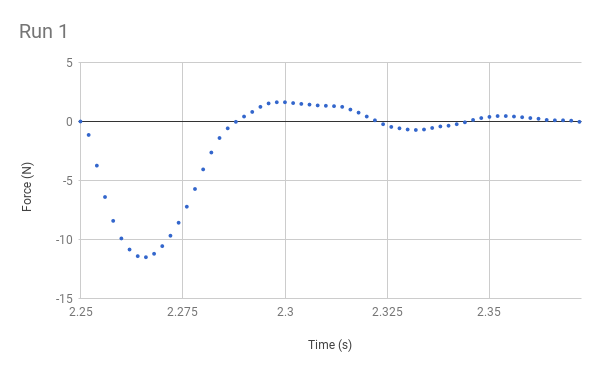
\includegraphics[scale=0.77]{images/08-impulse/run1.png}
    \end{center}
    \caption{}
\end{figure}
%%%%%%%%%%%%%%%%%%%%%%%%%%%%%%%%%%%%%%%%%%%%%%%%%%%%%%%%%%%%%%%%%%%%%%%%%%%%%%%%
\section{Your Data}
%%%%%%%%%%%%%%%%%%%%%%%%%%%%%%%%%%%%%%%%%%%%%%%%%%%%%%%%%%%%%%%%%%%%%%%%%%%%%%%%
You collected data for elastic collisions. Everyone is going to use the same data for the inelastic case.
%%%%%%%%%%%%%%%%%%%%%%%%%%%%%%%%%%%%%%%%%%%%%%%%%%%%%%%%%%%%%%%%%%%%%%%%%%%%%%%%
\section{Your Lab Report}
%%%%%%%%%%%%%%%%%%%%%%%%%%%%%%%%%%%%%%%%%%%%%%%%%%%%%%%%%%%%%%%%%%%%%%%%%%%%%%%%
In your lab report you should include:
\begin{enumerate}
    \item A table like table \ref{table.08.results.elastic} for both the elastic and the inelastic collisions. Use these tables to answer the questions below.
    \item A table like table \ref{table.08.results.inelastic} for both the elastic and the inelastic collisions.
    \item How does the average force during the elastic collisions compare to the average force during the inelastic collision?
    \item How does the collision duration $\Delta t$ for the elastic collisions compare to the inelastic collisions?
\end{enumerate}
% Copyright 2018 Melvin Eloy Irizarry-Gelpí
\chapter{Collisions and Momentum}
%%%%%%%%%%%%%%%%%%%%%%%%%%%%%%%%%%%%%%%%%%%%%%%%%%%%%%%%%%%%%%%%%%%%%%%%%%%%%%%%
...
%%%%%%%%%%%%%%%%%%%%%%%%%%%%%%%%%%%%%%%%%%%%%%%%%%%%%%%%%%%%%%%%%%%%%%%%%%%%%%%%
\section{Preliminary}
%%%%%%%%%%%%%%%%%%%%%%%%%%%%%%%%%%%%%%%%%%%%%%%%%%%%%%%%%%%%%%%%%%%%%%%%%%%%%%%%
...
%%%%%%%%%%%%%%%%%%%%%%%%%%%%%%%%%%%%%%%%%%%%%%%%%%%%%%%%%%%%%%%%%%%%%%%%%%%%%%%%
\section{Experiment}
%%%%%%%%%%%%%%%%%%%%%%%%%%%%%%%%%%%%%%%%%%%%%%%%%%%%%%%%%%%%%%%%%%%%%%%%%%%%%%%%
...
%%%%%%%%%%%%%%%%%%%%%%%%%%%%%%%%%%%%%%%%%%%%%%%%%%%%%%%%%%%%%%%%%%%%%%%%%%%%%%%%
\section{Analysis}
%%%%%%%%%%%%%%%%%%%%%%%%%%%%%%%%%%%%%%%%%%%%%%%%%%%%%%%%%%%%%%%%%%%%%%%%%%%%%%%%
...
%%%%%%%%%%%%%%%%%%%%%%%%%%%%%%%%%%%%%%%%%%%%%%%%%%%%%%%%%%%%%%%%%%%%%%%%%%%%%%%%
\section{My Data}
%%%%%%%%%%%%%%%%%%%%%%%%%%%%%%%%%%%%%%%%%%%%%%%%%%%%%%%%%%%%%%%%%%%%%%%%%%%%%%%%
...
%%%%%%%%%%%%%%%%%%%%%%%%%%%%%%%%%%%%%%%%%%%%%%%%%%%%%%%%%%%%%%%%%%%%%%%%%%%%%%%%
\section{Your Data}
%%%%%%%%%%%%%%%%%%%%%%%%%%%%%%%%%%%%%%%%%%%%%%%%%%%%%%%%%%%%%%%%%%%%%%%%%%%%%%%%
...
%%%%%%%%%%%%%%%%%%%%%%%%%%%%%%%%%%%%%%%%%%%%%%%%%%%%%%%%%%%%%%%%%%%%%%%%%%%%%%%%
\section{Your Lab Report}
%%%%%%%%%%%%%%%%%%%%%%%%%%%%%%%%%%%%%%%%%%%%%%%%%%%%%%%%%%%%%%%%%%%%%%%%%%%%%%%%
...
\chapter{Centripetal Motion}
%%%%%%%%%%%%%%%%%%%%%%%%%%%%%%%%%%%%%%%%%%%%%%%%%%%%%%%%%%%%%%%%%%%%%%%%%%%%%%%%%%%%%%%%%
...
%%%%%%%%%%%%%%%%%%%%%%%%%%%%%%%%%%%%%%%%%%%%%%%%%%%%%%%%%%%%%%%%%%%%%%%%%%%%%%%%%%%%%%%%%
\section{Preliminary}
%%%%%%%%%%%%%%%%%%%%%%%%%%%%%%%%%%%%%%%%%%%%%%%%%%%%%%%%%%%%%%%%%%%%%%%%%%%%%%%%%%%%%%%%%
...
%%%%%%%%%%%%%%%%%%%%%%%%%%%%%%%%%%%%%%%%%%%%%%%%%%%%%%%%%%%%%%%%%%%%%%%%%%%%%%%%%%%%%%%%%
\section{Experiment}
%%%%%%%%%%%%%%%%%%%%%%%%%%%%%%%%%%%%%%%%%%%%%%%%%%%%%%%%%%%%%%%%%%%%%%%%%%%%%%%%%%%%%%%%%
...
%%%%%%%%%%%%%%%%%%%%%%%%%%%%%%%%%%%%%%%%%%%%%%%%%%%%%%%%%%%%%%%%%%%%%%%%%%%%%%%%%%%%%%%%%
\section{Analysis}
%%%%%%%%%%%%%%%%%%%%%%%%%%%%%%%%%%%%%%%%%%%%%%%%%%%%%%%%%%%%%%%%%%%%%%%%%%%%%%%%%%%%%%%%%
...
%%%%%%%%%%%%%%%%%%%%%%%%%%%%%%%%%%%%%%%%%%%%%%%%%%%%%%%%%%%%%%%%%%%%%%%%%%%%%%%%%%%%%%%%%
\section{My Data}
%%%%%%%%%%%%%%%%%%%%%%%%%%%%%%%%%%%%%%%%%%%%%%%%%%%%%%%%%%%%%%%%%%%%%%%%%%%%%%%%%%%%%%%%%
...
%%%%%%%%%%%%%%%%%%%%%%%%%%%%%%%%%%%%%%%%%%%%%%%%%%%%%%%%%%%%%%%%%%%%%%%%%%%%%%%%%%%%%%%%%
\section{Your Data}
%%%%%%%%%%%%%%%%%%%%%%%%%%%%%%%%%%%%%%%%%%%%%%%%%%%%%%%%%%%%%%%%%%%%%%%%%%%%%%%%%%%%%%%%%
...
%%%%%%%%%%%%%%%%%%%%%%%%%%%%%%%%%%%%%%%%%%%%%%%%%%%%%%%%%%%%%%%%%%%%%%%%%%%%%%%%%%%%%%%%%
\section{Your Lab Report}
%%%%%%%%%%%%%%%%%%%%%%%%%%%%%%%%%%%%%%%%%%%%%%%%%%%%%%%%%%%%%%%%%%%%%%%%%%%%%%%%%%%%%%%%%
...
% Copyright 2018 Melvin Eloy Irizarry-Gelpí
\chapter{Simple Harmonic Motion}
%%%%%%%%%%%%%%%%%%%%%%%%%%%%%%%%%%%%%%%%%%%%%%%%%%%%%%%%%%%%%%%%%%%%%%%%%%%%%%%%
...
%%%%%%%%%%%%%%%%%%%%%%%%%%%%%%%%%%%%%%%%%%%%%%%%%%%%%%%%%%%%%%%%%%%%%%%%%%%%%%%%
\section{Preliminary}
%%%%%%%%%%%%%%%%%%%%%%%%%%%%%%%%%%%%%%%%%%%%%%%%%%%%%%%%%%%%%%%%%%%%%%%%%%%%%%%%
When an elastic spring is stretched or compressed beyond its natural relaxed length, a restorative force arises on the spring that causes the spring to return to its natural relaxed length. This force is proportional to how much distance $x$ the spring is stretched:
\begin{equation}
    F_{k} = - k x
    \label{eq.11.hooke}
\end{equation}
Here the minus sign is due to the restorative nature of the force (it is always opposite to what the spring is doing), and $k$ is the spring constant.

If a mass $m$ is attached to one end of the spring, the mass will move back-and-forth when the spring is stretched or compressed. Due to Newton's second law, you have a relation between force and acceleration:
\begin{equation}
    F_{\text{net}} = m a \quad \Longrightarrow \quad -kx = m a
\end{equation}
Or in other words:
\begin{equation}
    a = -\left( \frac{k}{m} \right) x
    \label{eq.11.ax}
\end{equation}
That is, for this motion, the acceleration is proportional to the amount of distance that the spring is stretched or compressed. Note that the slope is negative.

When you look at the position as it change with time, it follows a pattern similar to a sine or cosine function, familiar from trigonometry. This suggest a sinusoidal fit for position $x$ as a function of time $t$:
\begin{equation}
    x(t) = A \sin{\left( Bt + C \right)} + D
\end{equation}
Here $A$ is the amplitude of the motion (in m), $B$ is the angular frequency (in rad/s), $C$ is the time shift (in rad), and $D$ is the position shift (in m). Velocity is defined as the rate of change of position with respect to time. With calculus, this is equivalent to taking a derivative with respect to time:
\begin{equation}
    v(t) = \frac{\mathrm{d} x}{\mathrm{d} t} = AB \cos{\left( Bt + C \right)}
    \label{eq.11.v}
\end{equation}
That is, the parameters that describe the fit for position ($A$, $B$, $C$, and $D$) can also be used to describe the fit for velocity. Similarly, acceleration is defined as the rate of change of velocity with respect to time. With calculus, this is equivalent to taking a derivative with respect to time:
\begin{equation}
    a(t) = \frac{\mathrm{d} v}{\mathrm{d} t} = -AB^{2} \sin{\left( Bt + C \right)}
    \label{eq.11.a}
\end{equation}
Again, the parameters that describe the fit for position can also be used to describe the fit for acceleration.

For a mass $m$ attached to a spring with spring constant $k$, the period of oscillation is given by
\begin{equation}
    T = 2\pi \sqrt{\frac{m}{k}}
\end{equation}
The period is the time it takes for the mass to do one full cycle. Related to the period is the angular frequency $\omega$:
\begin{equation}
    \omega = \frac{2 \pi}{T} = \sqrt{\frac{k}{m}}
    \label{eq.11.omega}
\end{equation}
As you are going to see, the same value of angular frequency controls how quickly position, velocity, acceleration, and force change with time.
%%%%%%%%%%%%%%%%%%%%%%%%%%%%%%%%%%%%%%%%%%%%%%%%%%%%%%%%%%%%%%%%%%%%%%%%%%%%%%%%
\section{Experiment}
%%%%%%%%%%%%%%%%%%%%%%%%%%%%%%%%%%%%%%%%%%%%%%%%%%%%%%%%%%%%%%%%%%%%%%%%%%%%%%%%
We are going to use a motion sensor to measure the position, velocity and acceleration of a mass hanging from a spring. The spring in turn hangs from a force sensor that we are going to use to measure force. When the sensor is zeroed correctly, the constant weight force $mg$ is taken into account. When the hanging mass is moved from equilibrium and released, the motion is oscillatory.

After recording data for a short time, you can use the LabQuest device to obtain the values of the parameters $A$, $B$, $C$, and $D$ that best describe the force and the position data versus time.

We are going to do four combinations of mass and spring constant, as stated in Table \ref{table.11.parameters}.
%%%%%%%%%%%%%%%%%%%%%%%%%%%%%%%%%%%%%%%%%%%%%%%%%%%%%%%%%%%%%%%%%%%%%%%%%%%%%%%%
\begin{table}
	\begin{center}
		\begin{tabular}{|r|r|r|}\hline
			$k$ (N/m) & $m$ (kg) & $\omega$ (rad/s) \\ \hline
            5 & 0.05 & 10 \\
            5 & 0.1 & 7.071 \\
            15 & 0.1 & 12.247 \\
            15 & 0.15 & 10 \\
			\hline
		\end{tabular}
	\end{center}
	\caption{Four combinations of mass and spring constant, along with $\omega$ prediction}
	\label{table.11.parameters}
\end{table}
%%%%%%%%%%%%%%%%%%%%%%%%%%%%%%%%%%%%%%%%%%%%%%%%%%%%%%%%%%%%%%%%%%%%%%%%%%%%%%%%
\section{Analysis}
%%%%%%%%%%%%%%%%%%%%%%%%%%%%%%%%%%%%%%%%%%%%%%%%%%%%%%%%%%%%%%%%%%%%%%%%%%%%%%%%
There are many aspects of simple harmonic motion that can be verified with this experiment.
%%%%%%%%%%%%%%%%%%%%%%%%%%%%%%%%%%%%%%%%%%%%%%%%%%%%%%%%%%%%%%%%%%%%%%%%%%%%%%%%
\subsection{Force and Position}
%%%%%%%%%%%%%%%%%%%%%%%%%%%%%%%%%%%%%%%%%%%%%%%%%%%%%%%%%%%%%%%%%%%%%%%%%%%%%%%%
You can verify Hooke's law, equation (\ref{eq.11.hooke}), by making a scatter plot chart with position in the horizontal axis, and force in the vertical axis. The shape of this graph is a downward line, as in Figure \ref{figure.11.hooke}. You can find the slope with the \texttt{SLOPE} function. If position is in column X with the first value in row 6, and force is in column Y, with first value in row 6; then the command is
\begin{center}
    \texttt{=SLOPE(Y6:Y, X6:X)}
\end{center}
The linear behavior confirms Hooke's law. The slope of the linear fit corresponds to the (negative) value of the spring constant. Conversely, the negative of the slope serves as an indirect measurement of the spring constant:
\begin{equation}
    k_{\text{exp}} = - (\text{slope of force versus position linear fit})
\end{equation}
Note that position and force data come from different sensors.
%%%%%%%%%%%%%%%%%%%%%%%%%%%%%%%%%%%%%%%%%%%%%%%%%%%%%%%%%%%%%%%%%%%%%%%%%%%%%%%%
\begin{figure}
    \begin{center}
        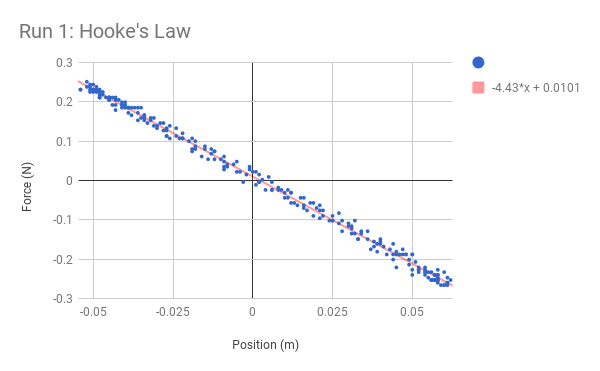
\includegraphics[scale=0.77]{images/11-shm/hooke.png}
    \end{center}
    \caption{}
    \label{figure.11.hooke}
\end{figure}
%%%%%%%%%%%%%%%%%%%%%%%%%%%%%%%%%%%%%%%%%%%%%%%%%%%%%%%%%%%%%%%%%%%%%%%%%%%%%%%%
\subsection{Force and Acceleration}
%%%%%%%%%%%%%%%%%%%%%%%%%%%%%%%%%%%%%%%%%%%%%%%%%%%%%%%%%%%%%%%%%%%%%%%%%%%%%%%%
You can verify Newton's second law of motion by making a scatter plot chart with acceleration in the horizontal axis, and force in the vertical axis. The shape of this graph is an upward line, as in Figure \ref{figure.11.newton}. You can find the slope with the \texttt{SLOPE} function. The linear behavior confirms Newton's second law, and the value of the slope is mass. You can use this slope as an indirect measurement of the amount of mass hanging from the spring:
\begin{equation}
    m_{\text{exp}} = \text{slope of force versus acceleration linear fit}
\end{equation}
Note that acceleration and force data come from different sensors.

Together with the measurement of the spring constant from the force versus position graph, you can compute an experimental estimate of the angular frequency via
\begin{equation}
    \omega_{1} = \sqrt{\frac{k_{\text{exp}}}{m_{\text{exp}}}}
\end{equation}
%%%%%%%%%%%%%%%%%%%%%%%%%%%%%%%%%%%%%%%%%%%%%%%%%%%%%%%%%%%%%%%%%%%%%%%%%%%%%%%%
\begin{figure}
    \begin{center}
        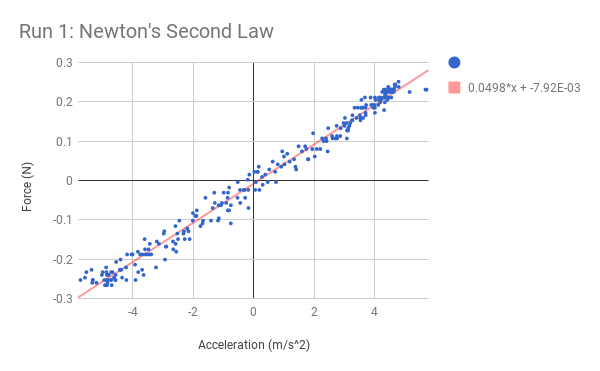
\includegraphics[scale=0.77]{images/11-shm/newton.png}
    \end{center}
    \caption{}
    \label{figure.11.newton}
\end{figure}
%%%%%%%%%%%%%%%%%%%%%%%%%%%%%%%%%%%%%%%%%%%%%%%%%%%%%%%%%%%%%%%%%%%%%%%%%%%%%%%%
\subsection{Acceleration and Position}
%%%%%%%%%%%%%%%%%%%%%%%%%%%%%%%%%%%%%%%%%%%%%%%%%%%%%%%%%%%%%%%%%%%%%%%%%%%%%%%%
Combining Hooke's law with Newton's second law of motion gives equation (\ref{eq.11.ax}). Using the definition of $\omega$ in equation (\ref{eq.11.omega}), we find that indeed,
\begin{equation}
    a = -\omega^{2}x
\end{equation}
That is, for simple harmonic motion, the acceleration is proportional to the position with the slope being the (negative) squared angular frequency. The shape of this graph is a downward line, as in Figure \ref{figure.11.ax}. The slope of this graph is the negative of the squared angular frequency. This value provides another experimental estimate of the angular frequency:
\begin{equation}
    \omega_{2} = \sqrt{- (\text{slope of acceleration versus position})}
\end{equation}
%%%%%%%%%%%%%%%%%%%%%%%%%%%%%%%%%%%%%%%%%%%%%%%%%%%%%%%%%%%%%%%%%%%%%%%%%%%%%%%%
\begin{figure}
    \begin{center}
        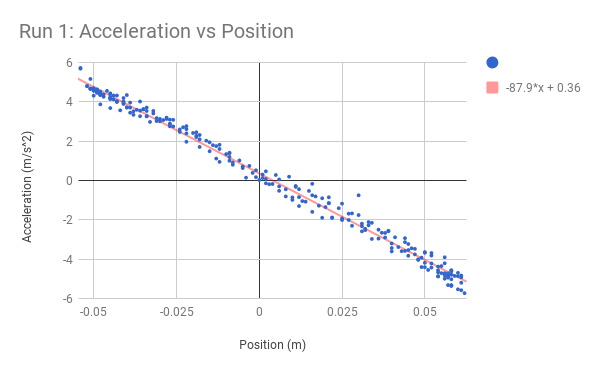
\includegraphics[scale=0.77]{images/11-shm/a-vs-x.png}
    \end{center}
    \caption{}
    \label{figure.11.ax}
\end{figure}
%%%%%%%%%%%%%%%%%%%%%%%%%%%%%%%%%%%%%%%%%%%%%%%%%%%%%%%%%%%%%%%%%%%%%%%%%%%%%%%%
\subsection{Common Angular Frequency}
%%%%%%%%%%%%%%%%%%%%%%%%%%%%%%%%%%%%%%%%%%%%%%%%%%%%%%%%%%%%%%%%%%%%%%%%%%%%%%%%
From the LabQuest device, you can obtain the parameters for the sinusoidal fit for position and force. The values for $A$, $C$, and $D$ will not necessarily agree, but the values for $B$ in both fits should be very close. Indeed, the $B$ from the force and position fits provide yet more experimental estimates of the angular frequency:
\begin{equation}
    \omega_{3} = B \text{ from force fit}
\end{equation}
and
\begin{equation}
    \omega_{4} = B \text{ from position fit}
\end{equation}
Note that, since the data for position and force comes from different sensors, these measurements can be taken as fully independent.

In principle you can perform a sinusoidal fit on velocity and acceleration too. However, the parameters of these fits are not independent. Indeed, theoretically, they depend on the parameters for the position fit as stated in equations (\ref{eq.11.v}) and (\ref{eq.11.a}). In class we saw how you can use compute the fit functions in (\ref{eq.11.v}) and (\ref{eq.11.a}) with the parameters from the position fit, and how those function are in very good agreement with the experimental data collected.
%%%%%%%%%%%%%%%%%%%%%%%%%%%%%%%%%%%%%%%%%%%%%%%%%%%%%%%%%%%%%%%%%%%%%%%%%%%%%%%%
\subsection{Velocity and Position}
%%%%%%%%%%%%%%%%%%%%%%%%%%%%%%%%%%%%%%%%%%%%%%%%%%%%%%%%%%%%%%%%%%%%%%%%%%%%%%%%
A graph with velocity and position is called a phase space graph. For this particular experiment with simple harmonic motion, the velocity and position data yield an elliptical shape (a closed orbit), as in Figure \ref{figure.11.phase}. Now you know!
%%%%%%%%%%%%%%%%%%%%%%%%%%%%%%%%%%%%%%%%%%%%%%%%%%%%%%%%%%%%%%%%%%%%%%%%%%%%%%%%
\begin{figure}
    \begin{center}
        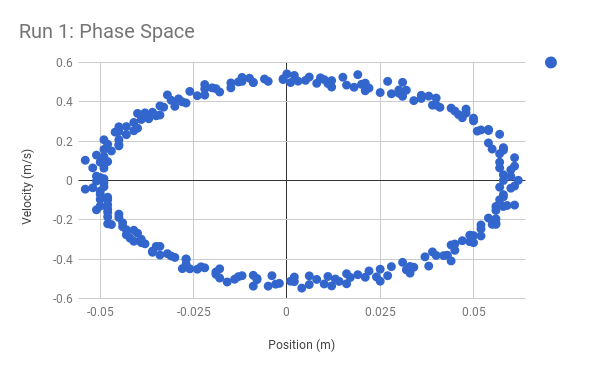
\includegraphics[scale=0.77]{images/11-shm/phase.png}
    \end{center}
    \caption{}
    \label{figure.11.phase}
\end{figure}
%%%%%%%%%%%%%%%%%%%%%%%%%%%%%%%%%%%%%%%%%%%%%%%%%%%%%%%%%%%%%%%%%%%%%%%%%%%%%%%%
\section{My Data}
%%%%%%%%%%%%%%%%%%%%%%%%%%%%%%%%%%%%%%%%%%%%%%%%%%%%%%%%%%%%%%%%%%%%%%%%%%%%%%%%
The results for my run 1 are summarized in Table \ref{table.11.results}.
%%%%%%%%%%%%%%%%%%%%%%%%%%%%%%%%%%%%%%%%%%%%%%%%%%%%%%%%%%%%%%%%%%%%%%%%%%%%%%%%
\begin{table}
    \begin{center}
        \begin{tabular}{|l|r|}
            \hline
            Name & Value \\
            \hline
            $m_{\text{exp}}$ & 0.0498 kg \\
            $k_{\text{exp}}$ & 4.4255 N/m \\
            $\omega_{1}$ & 9.4230 rad/s \\
            $\omega_{2}$ & 9.3776 rad/s \\
            $\omega_{3}$ & 9.5802 rad/s \\
            $\omega_{4}$ & 9.5796 rad/s \\
            \hline
            $\omega_{\text{ave}}$ & 9.4901 rad/s \\
            \hline
        \end{tabular}
    \end{center}
    \caption{Results for run 1. The last row is the average of the previous four rows.}
	\label{table.11.results}
\end{table}
%%%%%%%%%%%%%%%%%%%%%%%%%%%%%%%%%%%%%%%%%%%%%%%%%%%%%%%%%%%%%%%%%%%%%%%%%%%%%%%%
\section{Your Data}
%%%%%%%%%%%%%%%%%%%%%%%%%%%%%%%%%%%%%%%%%%%%%%%%%%%%%%%%%%%%%%%%%%%%%%%%%%%%%%%%
...
%%%%%%%%%%%%%%%%%%%%%%%%%%%%%%%%%%%%%%%%%%%%%%%%%%%%%%%%%%%%%%%%%%%%%%%%%%%%%%%%
\section{Your Lab Report}
%%%%%%%%%%%%%%%%%%%%%%%%%%%%%%%%%%%%%%%%%%%%%%%%%%%%%%%%%%%%%%%%%%%%%%%%%%%%%%%%
In your lab report you should include:
\begin{enumerate}
    \item A version of Table \ref{table.11.results} with four runs, one for each different mass/spring constant combination. You do not have to make the graphs in order to get the slopes; use the \texttt{SLOPE} function.
    \item One acceleration versus position graph with the linear fit, for a run of your choosing.
    \item One force versus acceleration graph with the linear fit, for a run of your choosing.
    \item One force versus position graph with the linear fit, for a run of your choosing.
    \item One velocity versus position graph for a run of your choosing.
\end{enumerate}
You should answer the following questions:
\begin{enumerate}
    \item Based on your analysis and what we saw in class, are you convinced that (for simple harmonic motion) all of position, velocity, acceleration, and force can be described by sines or cosines with a common angular frequency?
    \item Is the angular frequency parameter $B$ for the position versus time graph the same or close to the angular frequency parameter $B$ for the force versus time graph?
    \item Can you test Newton's second law with the data from this experiment? Does the measured mass agree with the expected value used?
    \item Can you test Hooke's law with the data from this experiment? Does the measured spring constant agree with the expected value used?
    \item Are your four estimates of the angular frequencies close to the expected theoretical value given by (\ref{eq.11.omega}).
\end{enumerate}
%%%%%%%%%%%%%%%%%%%%%%%%%%%%%%%%%%%%%%%%%%%%%%%%%%%%%%%%%%%%%%%%%%%%%%%%%%%%%%%%%%%%%%%%%
\end{document}